%Basic Formatting and Packages---------------------------------------------------------------------------------------------------------------------------------------------------------------------------
\documentclass[11pt,a4paper]{article}
\usepackage{amsmath} 
\usepackage{amssymb}
\usepackage{bm}
\usepackage{graphicx}
\usepackage{geometry}
\usepackage{mathtools}
\usepackage[dvipsnames]{xcolor}
\usepackage{enumitem}
\usepackage{tcolorbox}
\usepackage{verbatim}
\usepackage{csvsimple}
\usepackage{subcaption}
\usepackage[font=tiny,labelfont=bf]{caption}
\usepackage{float}
\usepackage{listings}
\usepackage{hyperref}

\usepackage{longtable}
\usepackage{multirow}
\usepackage{array}
\usepackage{booktabs}
\usepackage[ruled, noend]{algorithm2e}

\usepackage{tikz}
\usetikzlibrary{shapes, shapes.geometric, positioning, arrows.meta, fit, snakes, calc, graphs, graphs.standard}

\geometry{left=2cm,right=2cm,top=2.5cm,bottom=2.5cm}


\lstset{basicstyle=\footnotesize}



\title{\textbf{Likelihood Estimation Comparison for Energy Based Models: A Framework}}
    \author{
        \parbox{\linewidth}{\centering
            Manuel Günther
        }
     }
    \date{\today}

\usepackage{newunicodechar}
\newunicodechar{⁠}{\nolinebreak}




\definecolor{myblue}{cmyk}{1,.72,0,.38}

% Define custom colors
%\definecolor{myblue}{rgb}{0,0,1}
\definecolor{myyellow}{rgb}{1,1,0}
\definecolor{myorange}{rgb}{1,0.5,0}
\definecolor{mypurple}{rgb}{0.5,0,0.5}
\definecolor{mygreen}{rgb}{0,0.5,0}

%Python code style settings---------------------------------------------------------------------------------------------------------------------------------------------------------------------------------------

% Define a custom style for Python code
\lstdefinestyle{mystyle}{
    backgroundcolor=\color{white},       % background color
    commentstyle=\color{mygreen},        % comment color
    keywordstyle=\color{mypurple},         % keyword color
    numberstyle=\tiny\color{gray},     % line numbers color
    stringstyle=\color{orange},       % string color 
    identifierstyle =\color{myblue},
    basicstyle=\ttfamily\scriptsize,          % code font and size
    breakatwhitespace=false,             % break lines only at whitespace
    breaklines=true,                     % enable line breaking
    captionpos=b,                        % caption position (bottom)
    keepspaces=true,                     % keep spaces in code
    numbers=left,                        % line numbers position (left)
    numbersep=5pt,                       % distance between line numbers and code
    %numbers=none,                        % line numbers position (left)
    showspaces=false,                    % show spaces using underscores
    showstringspaces=false,              % show spaces in strings as underscores
    showtabs=false,                      % show tabs using underscores
    tabsize=4                            % tab size
}

% Set custom colors for specific keywords and function names
\lstset{
    language=Python,
    style=mystyle,
    %morekeywords={class, def},   % Add keywords to highlight
    %keywordstyle=\color{myblue}, % Keyword color
    %morekeywords={for, in},
    %keywordstyle=\color{mypurple}, % Keywords "for" and "in" will be purple       
    emph={max, min, sum},                  % Define function name(s) to highlight
    emphstyle=\color{Goldenrod},          % Function name color
    %emph={for, in},                  % Define function name(s) to highlight
    %emphstyle=\color{mypurple},          % Function name color
}


%Own Commands----------------------------------------------------------------------------------------------------------------------------------------------------------------------------------------------------
%1. Inequality in set: ieset
%Default: lhs is tau
\newcommand{\ieset}[2][\tau]{\{#1 \le #2\}} 
%Example: to get {X <= t} use this expression $\ieset[X]{t}$

%2. Expectation: Ex
\newcommand{\Ex}[1]{ \mathbb{E}\left[ #1 \right] }
%Example: to get E[ X ] use this expression $\Ex{X}$

%3. In curly brackets: icb
\newcommand{\icb}[1]{\{ #1 \}}
%Example: to get {a = b} use this expression $\icb{a = b}

%4. Norm: norm
%\newcommand{\norm}[1]{\left\lVert#1\right\rVert}
\newcommand{\norm}[2][2]{\left\lVert#2\right\rVert_{#1}}
%Example: to get ||X|| use the expression \norm{X}

%5. Column Vector
\newcommand*\colvec[1]{\begin{pmatrix}#1\end{pmatrix}}
%Example: \colvec{a \\ b} gives vector (a,b) transposed.

%6.Row Vector
\newcommand{\rvec}[1]{\begin{bmatrix} #1 \end{bmatrix}}
%Example: \rvect{a & b} gives vector (a,b)

%7. Abs:
\newcommand{\abs}[1]{\left |#1\right|}
%Example: to get |X| use the expression \abs{X}

\newcommand*\dif{\mathop{}\!\mathrm{d}}


%Own Paired Delimiter----------------------------------------------------------------------------------------------------------------------------------------------------------------------------------------------------

% Variation of latex code from https://tex.stackexchange.com/questions/389450/scaling-of-langle-and-rangle-for-large-enclosed-symbols
% Would allow to write single entry Or comma separated argument which would automatically convert
% Uses package: \usepackage{xparse, etoolbox}

\DeclarePairedDelimiterX{\Innerp}[1]{\langle}{\rangle}{\Innpargs{#1}}

\NewDocumentCommand{\Innpargs}{>{\SplitArgument{1}{,}}m}{\Innpargsaux#1}

\NewDocumentCommand{\Innpargsaux}{mm}
{
	\IfNoValueTF{#2}
		{\IfNoValueTF{#1}
			{\, \cdot \,{,}\, \cdot \,} % Both arguments have no value
			{{ #1 \,}{,}{\, #1}} % Only the first argument given
		}
		{{#1\,} {,} \, #2} % Both arguments given
}%


%Own Operators----------------------------------------------------------------------------------------------------------------------------------------------------------------------------------------------------
\DeclareMathOperator*{\argmax}{arg\,max}
\DeclareMathOperator*{\argmin}{arg\,min}

\DeclareMathOperator*{\curl}{curl}

\let\div\relax %remove the existing div command to allow operator definition
\DeclareMathOperator*{\div}{div}

\DeclareMathOperator*{\grad}{grad}

%Redeclared Operators----------------------------------------------------------------------------------------------------------------------------------------------------------------------------------------------------
\let\bar\overline
\let\ul\underline
\let\del\partial



% Redefining single $...$ inline math------------------------------------------------------------------------------------------------------------------------------------------------------------------
\let\originalmathdollar=$
\catcode`\$=\active
\def$#1${\originalmathdollar\color{myblue}#1\originalmathdollar}

% Redefining the display math environment ------------------------------------------------------------------------------------------------------------------------------------------------------------------
% Save the original definition of the display math environment
\let\originaldisplaymath=\[
\let\endoriginaldisplaymath=\]

% Redefine the display math environment to include color
\renewcommand{\[}{\begin{originaldisplaymath}\color{myblue}}
\renewcommand{\]}{\end{originaldisplaymath}}



% Redefining the equation environment ------------------------------------------------------------------------------------------------------------------------------------------------------------------
% Save the original definition of the equation environment
\let\originalequation=\equation
\let\endoriginalequation=\endequation

% Redefine the equation environment to include color
\renewenvironment{equation}{\begin{originalequation}\color{myblue}}{\end{originalequation}}


\setlength{\parindent}{0pt}
%\setlength{\parskip}{2pt}







\begin{document}
%Inputs from content----------------------------------------------------------------------------------------------------------------------------------------------------------------------------------------------------

\maketitle
\tableofcontents

\section{Introduction}

Energy based models are widely used in statistical learning and can also be found as elegant models of spatial interactions in point process models. 
However, maximum likelihood (ML) based inference usually remains challenging due to the difficulty in approximating the partition function using Markov Chain Monte Carlo (MCMC) for high- dimensional multimodal distributions.

Following the work of Gao and Song(\cite{Gao-Song2020}), the goal of this project is to explore the efficacy and efficiency of recovery likelihood estimation in learning parametrised models.
The RL approach is based on applying Gaussian noise to the training data and subsequently using the conditional instead of the marginal distribution.
We will shown that this approach yields an unbiased estimator of the underlying parameters and investigate the MCMC sampling properties. 

As the inference process depends on many components and hyperparameters, comparing these estimators empirically is necessarily not comprehensive.
Depending on the training data, the model used, the sampling approach and components like the optimiser, the results might be different.
Thus a large part of this project was dedicated to develop a general code framework that allows for more systematic testing in a setting of interest.

 have shown that RL produces good results and computational savings in the context of image generation.
In that context and many others the models are typically some variety of neural networks.
For neural network architectures the concrete values of the weights and biases are less significant, 
and two architectures with fundamentally different parameter values can still produce similar distributions.
In this project the emphasis is on parametric models whose parameters carry a direct meaning or function as the basis for further analysis.
For such models it is not just important that the resulting distribution coincides with the data distribution, 
but also that the parameters themselves are estimated accurately.
The later comparisons will hence focus primarily on how well the estimated parameters match the distribution parameters.

\subsection{Problem Formulation}
The problem that is investigated in statistical learning of generative models looks like this:
We have a dataset $\mathcal{D} = (\bm{x}_i)_{i = 1}^n \subseteq \mathbb{R}^d$ from an unknown distribution of a random vector $\bm{X} : \Omega \to \mathbb{R}^d$,
with some probability density function $p : \mathbb{R}^d \to \mathbb{R}$.
We want to use the data to approximate this density function with a parametrised model density function $p_{\bm{\theta}}: \mathbb{R}^d \to \mathbb{R}$,
for a vector of parameters $\bm{\theta} \in \mathbb{R}^m$, by estimating an optimal $\hat{\bm{\theta}}$ such that $p_{ \hat{\bm{\theta}} }$ is close to $p$.


\subsection{Approaches}
For high dimensional multimodal problems and complicated target densities $p$ estimating $\hat{\bm{\theta}}$ is a highly non-trivial task, 
where the standard ML inference can be computationally infeasible.
Complicating the problem further is that the model distributions need to be sufficiently complex to be able to resemble the target distribution and thus even the model
density is often only determined by its probability kernel, as the normalisation constant is not available analytically and costly to calculate numerically.

There are various approaches that attempt to make this inference problem tractable, such as 

\begin{comment}
\\
Denoising Diffusion Probabilistic Models

\\
Score Matching: 
(Estimation of Non-Normalized Statistical Models by Score Matching, Aapo Hyvarinen 2005)
- always at least locally consistent
-the model pdf needs to be smooth enough

\\
Pseudo-Likelihood Estimation: 
(Besag, Spatial interaction and the statistical analysis of lattice systems. Journal of the Royal Statistical Society, Series B, 36(2):192–236, 1974)
However, the conditional probabilities in (13) are not necessarily readily available and need to be computed. In particular, these conditional densities need to be normalized. The computational burden needed in the normalization is reduced from the original problem since we only need to numerically compute n one-dimensional integrals which is far more feasible than a single n-dimensional integral. However, compared to score matching, this is a computationally expensive method since score matching avoids the need for numerical integration altogether.
The question of consistency of pseudo-likelihood estimation seems to be unclear (in general).

\\
Contrastive Divergence (Hinton Training products of experts by minimizing contrastive divergence. Neural Computation, 14(8):1771–1800, 2002.)
he basic principle is to use an MCMC method for computing the derivative of the logarithm of the normalization factor Z, but the MCMC is allowed to run for only a single iteration (or a few iterations) before doing the gradient step.
- generally biased, even asymptotically
-much more general method than score matching since it is applicable to intractable latent variable models.
-can also handle binary/discrete variables

\end{comment}

%
\begin{comment}
We have a dataset $\mathcal{D} = (\bm{x}_i)_{i = 1}^n \subseteq \mathbb{R}^d$ from an unknown distribution of a random vector $\bm{X} : \Omega \to \mathbb{R}^d$,
with some probability density function $p : \mathbb{R}^d \to \mathbb{R}$.
We want to use the data to approximate this density function with a parametrised model density function $p_{\bm{\theta}}: \mathbb{R}^d \to \mathbb{R}$,
for a vector of parameters $\bm{\theta} \in \mathbb{R}^m$, by estimating an optimal $\hat{\bm{\theta}}$ such that $p_{ \hat{\bm{\theta}} }$ is close to $p$.
\end{comment}

\newtheorem{theorem}{Theorem}

\section{Score Matching}

Suppose we use a parametrised model density function $p_{\bm{\theta}}: \mathbb{R}^d \to \mathbb{R}$, 
for which we only know the probability kernel $K_{\bm{\theta}}: \mathbb{R}^d \to \mathbb{R}$ but not the normalisation constant $Z(\bm{\theta})$.

Score matching is based on minimising the expected square distance between the model score function and the data score function.
The model score function is defined as
\[
	S_{\bm{\theta}} (\bm{x}) = \nabla_{\bm{x}} \log p_{\bm{\theta}}(\bm{x})
\]

and similarly the data score function is given by
\[
	S (\bm{x}) = \nabla_{\bm{x}} \log p(\bm{x}).
\]

A major benefit of working with the score functions instead of with the densities directly is that the normalisation constant falls away,
\[
\begin{aligned}
	S_{\bm{\theta}} (\bm{x}) 
	&= \nabla_{\bm{x}} \log p_{\bm{\theta}}(\bm{x}) \\
	&= \nabla_{\bm{x}} \log \frac{ K_{\bm{\theta}}(\bm{x}) }{ Z(\bm{\theta}) } \\
	&= \nabla_{\bm{x}} \left( \log K_{\bm{\theta}}(\bm{x}) - \log Z(\bm{\theta}) \right) \\
	&= \nabla_{\bm{x}} \log K_{\bm{\theta}}(\bm{x}) \\
\end{aligned}
\]

such that knowing the kernel is sufficient for all involved calculations.
The objective function $J$, i.e. the expected square distance between the model score function and the data score function, is defined by
\[
	J(\bm{\theta}) = \frac{1}{2} \int_{\mathbb{R}^d} p(\bm{x}) \norm{ S_{\bm{\theta}} (\bm{x}) - S (\bm{x}) }^2 \dif \bm{x}
\]

and the estimator is then given by
\[
	\hat{\bm{\theta}} = \argmin_{\bm{\theta}} J(\bm{\theta})
\]

Up until this point we replaced one problem with another, as we might have to compute an estimator of the data score function $S$ from the observed sample, 
which is basically a non-parametric estimation problem.
However, when the following conditions are fulfilled:
\begin{enumerate}
	\item $S_{\bm{\theta}}$ is sufficiently differentiable
	\item $p$ is sufficiently differentiable
	\item $\forall \bm{\theta}: \quad \Ex{ \norm{ S_{\bm{\theta}}(\bm{X}) }^2 } < \infty $
	\item $\Ex{ \norm{ S(\bm{X}) }^2 } < \infty $
	\item $\forall \bm{\theta}: \quad \lim_{\norm{\bm{x}} \to \infty} p(\bm{x}) S_{\bm{\theta}}(\bm{x}) = 0$
\end{enumerate}

then the objective function can be represented without $S$ by the following theorem:

\begin{theorem}
Under the regularity conditions above, and denoting by $S_j^{\bm{\theta}}$ the $j$-th component of $S_{\bm{\theta}}$, the objective function $J$ can be expressed as
\[
	J(\bm{\theta}) = \int_{\mathbb{R}^d} p(\bm{x}) \sum_{j = 1}^d \left[ \del_j S_j^{\bm{\theta}} (\bm{x}) + \frac{1}{2} S_j^{\bm{\theta}}(\bm{x})^2 \right] \dif \bm{x} + C
\]

where the constant $C$ does not depend on $\bm{\theta}$,
\[
	S_j^{\bm{\theta}} (\bm{x}) = \frac{\del \log K_{\bm{\theta}}(\bm{x}) }{\del \bm{x}_j }
\]
and 
\[
	\del_j S_j^{\bm{\theta}} (\bm{x}) = \frac{\del S_j^{\bm{\theta}} (\bm{x}) }{\del \bm{x}_j } = \frac{\del^2 \log K_{\bm{\theta}}(\bm{x}) }{\del \bm{x}_j^2 }
\]
is the partial derivative of the model score function with respect to $\bm{x}_j$.
\end{theorem}

In practice, with the dataset $\mathcal{D}$ of $n$ observations of the random vector $\bm{X}$, denoted now as $(\bm{x}( i ) )_{i = 1}^n$ to avoid confusion, 
the sample version of $J$ is obtained from this as
\[
	\tilde{J}(\bm{\theta}) = \frac{1}{n} \sum_{i = 1}^n \sum_{j = 1}^d \left[ \del_j S_j^{\bm{\theta}} ( \bm{x}(i) ) + \frac{1}{2} S_j^{\bm{\theta}}( \bm{x}(i) )^2 \right] + C
\]

which is asymptotically equivalent to $J$ due to the law of large numbers. 
So one estimates the model by minimisation of $\tilde{J}$ in the case of a real, finite sample.

If we assume that the model is not degenerate, and that $K_{\bm{\theta}} > 0$ always, we have local consistency as shown by the following theorem and the corollary:

\begin{theorem}
Assume the probability density function of $\bm{X}$ follows the model $p(\cdot) = p_{\bm{\theta}^\ast}(\cdot)$ for some $\bm{\theta}^\ast$.
Assume further that $\bm{\theta}^\ast$ is unique in this role and that $\forall \bm{\theta}, \bm{x}: \quad K_{\bm{\theta}}(\bm{x}) > 0$, then
\[
	J(\bm{\theta}) = 0 \quad \Leftrightarrow \quad \bm{\theta} = \bm{\theta}^\ast
\]
\end{theorem}

Under the assumptions of the preceding Theorems, the score matching estimator obtained by minimisation of $\tilde{J}$ is consistent, 
i.e. it converges in probability towards the true value of $\bm{\theta}$ when sample size approaches infinity, 
assuming that the optimisation algorithm is able to find the global minimum.
In practice, this may not be true, in particular because there may be several local minima. 
Then, the consistency is of local nature, i.e., the estimator is consistent if the optimisation iteration is started sufficiently close to the true value. 
Note that consistency implies asymptotic unbiasedness.









\begin{comment}
Let $\bm{x} \sim p_{\text{data}}(\bm{x})$ denote a training example, and $p_{\bm{\theta}}(\bm{x})$ denote a model’s probability density function 
that aims to approximates $p_{\text{data}}(\bm{x})$. 
\end{comment}


\section{Energy Based Models}

For a function $U_{\bm{\theta}} : \mathbb{R}^d \to \mathbb{R}$, also called (potential) energy functional, an energy-based model (EBM) is defined as:

\[
	p_{\bm{\theta}} (\bm{x}) = \frac{1}{ Z_{\bm{\theta}} } \exp( - U_{\bm{\theta}} (\bm{x}) )
\]

where $Z_{\bm{\theta}} = \int \exp( - U_{\bm{\theta}} (\bm{x}) ) \dif \bm{x}$ is the partition function which is analytically intractable for high dimensional $\bm{x}$.



\subsection{Tranformation}
Any standard distribution for a random variable or vector $\bm{X} : \Omega \to \mathbb{R}^d$ with a continuous density $f_{\bm{X}}$ can be transformed into an EBM.
For this, an analytical representation of the probability kernel $K_{\bm{X}}$ of the distribution, i.e. the un-normalised version of the density, is already sufficient, 
making it an excellent tool for Bayesian models where the normalisation constant of the posterior is typically analytically unavailable or intractable.
Given the kernel we can set 
\[
	U(\bm{x}) = - \log K_{\bm{X}} (\bm{x}),
\]

which reproduces the desired density when substituted in the EBMs density form:

\[
\begin{aligned}
	p (\bm{x}) &= \frac{1}{ Z } \exp( - U(\bm{x}) ) \\
	&= \frac{1}{ \int \exp( - U (\bm{x}) ) \dif \bm{x} } \exp( - U(\bm{x}) ) \\
	&= \frac{1}{ \int \exp( \log K_{\bm{X}} (\bm{x}) ) \dif \bm{x} } \exp( \log K_{\bm{X}} (\bm{x}) ) \\
	&= \frac{1}{ \int K_{\bm{X}} (\bm{x}) \dif \bm{x} } K_{\bm{X}} (\bm{x}) \\
	&= f_{\bm{X}} (\bm{x}) \\
\end{aligned}
\]

We might not have an analytical representation for density or kernel but only a way of calculating the density value.
For analytical consideration it is helpful to be able to still have a representation for the energy functional.
We know that for a model with parameterised density $p_{\bm{\theta}}$ we have
\[
\begin{aligned}
	- \log p_{\bm{\theta}} (\bm{x}) 
	&= - \log \frac{ K_{\bm{\theta}} (\bm{x}) }{ Z_{\bm{\theta}} } \\
	&= - \log K_{\bm{\theta}} (\bm{x}) + \log Z_{\bm{\theta}}  \\
\end{aligned}
\]

so we can represent the energy functional as
\[
	U_{\bm{\theta}} (\bm{x}) = - \log p_{\bm{\theta}} (\bm{x}) - \log Z_{\bm{\theta}}
\]



\subsection{Differentiating}
For sampling and estimation we will have to differentiate the energy functional of a model by both the input $\bm{x}$ and by the parameter vector $\bm{\theta}$.

In general, for a function $f : \mathbb{R}^d \to \mathbb{R}$ we have by the chain rule that
\[
	\nabla_{\bm{x}} (- \log f(\bm{x}) ) = - \frac{ 1 }{ f(\bm{x}) } \nabla_{\bm{x}} f(\bm{x}) = - \frac{ \nabla_{\bm{x}} f(\bm{x}) }{ f(\bm{x}) } 
\]

so for a model were we have the kernel analytically the derivative with respect to $\bm{x}$ is
\[
\begin{aligned}
	\nabla_{\bm{x}} U_{\bm{\theta}} (\bm{x})
	&= \nabla_{\bm{x}} ( - \log K_{\bm{\theta}} (\bm{x}) ) \\
	&= - \frac{ \nabla_{\bm{x}} K_{\bm{\theta}} (\bm{x}) }{ K_{\bm{\theta}} (\bm{x}) }   \\
\end{aligned}
\]

and analogously for $\bm{\theta}$:
\[
	\nabla_{\bm{\theta}} U_{\bm{\theta}} (\bm{x}) = - \frac{ \nabla_{\bm{\theta}} K_{\bm{\theta}} (\bm{x}) }{ K_{\bm{\theta}} (\bm{x}) }.
\]

In the other case where we don't have the kernel explicitly the calculation is similar with respect to $\bm{x}$ as the normalisation constant falls away
\[
\begin{aligned}
	\nabla_{\bm{x}} U_{\bm{\theta}} (\bm{x})
	&= \nabla_{\bm{x}} ( - \log p_{\bm{\theta}} (\bm{x}) - \log Z_{\bm{\theta}} ) \\
	&=  - \nabla_{\bm{x}} \log p_{\bm{\theta}} (\bm{x}) - \nabla_{\bm{x}} \log Z_{\bm{\theta}} \\
	&= - \frac{ \nabla_{\bm{x}} p_{\bm{\theta}} (\bm{x}) }{ p_{\bm{\theta}} (\bm{x}) }  \\
\end{aligned}
\]

but more difficult when differentiating with respect to $\bm{\theta}$ as $Z_{\bm{\theta}}$ is a function of it.
\[
\begin{aligned}
	\nabla_{\bm{\theta}} U_{\bm{\theta}} (\bm{x})
	&= \nabla_{\bm{\theta}} ( - \log p_{\bm{\theta}} (\bm{x}) - \log Z_{\bm{\theta}} ) \\
	&=  - \nabla_{\bm{\theta}} \log p_{\bm{\theta}} (\bm{x}) - \nabla_{\bm{\theta}} \log Z_{\bm{\theta}} \\
	&= - \frac{ \nabla_{\bm{\theta}} p_{\bm{\theta}} (\bm{x}) }{ p_{\bm{\theta}} (\bm{x}) } - \frac{ \nabla_{\bm{\theta}} Z_{\bm{\theta}} }{ Z_{\bm{\theta}} }\\
\end{aligned}
\]
















\section{Test Distributions}

The models corresponding to the distributions, that are introduced in the following, will be explored in the experiments in the results section.
This is just a small selection, that will not cover many interesting questions or potential test cases, 
so the reader is invited to customise the framework, introduced later in this report, by adding a new model they consider interesting.
In the following, let $X: \Omega \to \mathbb{R}$ or $\bm{X}: \Omega \to \mathbb{R}^d$ be a random variable or a random vector respectively,
with the respective distribution.


\subsection{Multivariate Normal Distribution}

The multivariate normal distribution is a great place to start as it is ubiquitous, easy to handle and serves as a base component for many complex models and algorithms.
For mean $\bm{\mu} \in \mathbb{R}^d$ and covariance $\Sigma \in \mathbb{R}^{d \times d}$ we say $X$ follows a multivariate Gaussian 
or normal distribution $X \sim \mathcal{N}(\bm{\mu}, \Sigma)$, if its probability density function is given by:
%\textbf{Probability Density Function (pdf):}
\[
	f_X(\bm{x} | \bm{\mu}, \Sigma) = \frac{1}{(2\pi)^{n/2}|\Sigma|^{1/2}} \exp\left(-\frac{1}{2} (\bm{x} - \bm{\mu})^T \Sigma^{-1} (\bm{x} - \bm{\mu})\right)
\]

From this density one can obtain several components used later in sampling and estimation:
\textbf{Kernel:}
\[
	K_X (\bm{x}) = \exp \left( -\frac{1}{2} (\bm{x} - \bm{\mu})^T \Sigma^{-1} (\bm{x} - \bm{\mu}) \right)
\]

\textbf{Energy Function:}
\[
\begin{aligned}
	U(\bm{x}) &= - \log( K_X (\bm{x}) ) \\
	&= - \log( \exp \left( -\frac{1}{2} (\bm{x} - \bm{\mu})^T \Sigma^{-1} (\bm{x} - \bm{\mu}) \right) ) \\
	&= \left( \frac{1}{2} (\bm{x} - \bm{\mu})^T \Sigma^{-1} (\bm{x} - \bm{\mu}) \right)
\end{aligned}
\]

\textbf{Gradient of Energy Function with respect to $\bm{x}$:}
\[
\begin{aligned}
	\nabla U(\bm{x}) &= \nabla \left( \frac{1}{2} (\bm{x} - \bm{\mu})^T \Sigma^{-1} (\bm{x} - \bm{\mu}) \right) \\
	&= \Sigma^{-1} (\bm{x} - \bm{\mu}) \\
\end{aligned}
\]

\textbf{Gradient of Energy Function with respect to $\bm{\mu}$:}
\[
\begin{aligned}
	\nabla_{\bm{\mu}} U(\bm{x}) &= \nabla_{\bm{\mu}} \left( \frac{1}{2} (\bm{x} - \bm{\mu})^T \Sigma^{-1} (\bm{x} - \bm{\mu}) \right) \\
	&= \Sigma^{-1} (\bm{\mu} - \bm{x}) \\
\end{aligned}
\]

The partial derivatives of the energy functional with respect to $\Sigma_{i,j}$ however are not directly obtainable as there is no general form of $\Sigma^{-1}$ available.
Fortunately the gradient with respect to $\Sigma$ can still be obtained effectively with automatic differentiation, that is leveraged by the employed framework.


\subsection{Gaussian Mixture Distribution (GMD)}

Gaussian mixture distributions make for simple but sufficiently complex distribution for our parameter estimation testing process.
A GMD is a random vector  $\bm{X} : \Omega \to \mathbb{R}^d$, whose density is the weighted sum of the densities $f_i : \mathbb{R}^d \to \mathbb{R}$, 
of $m$ Gaussian random vectors $\bm{Z}_i \sim \mathcal{N}(\bm{\mu}_i , \Sigma_i )$ with corresponding weights $w_i \in (0, 1)$ such that $\sum_{i = 1}^m w_i$.
The density is given by
\[
	p_{\bm{\theta}} (\bm{x}) := \sum_{i = 1}^m w_i f_i(\bm{x})
\]

where the weights, means and covariances are aggregated in the parameter $\bm{\theta}$ for convenience.
For each $i \in [m]$ the density $f_i$ can be split in two parts, namely the kernel, which is denoted as $K_i$, and the normalisation constant $Z_i$, i.e.
\[
	f_i (\bm{x}) 
	= \underbrace{ \frac{1}{\sqrt{(2\pi)^{d} |\Sigma_i |}} }_{=: Z_i} 
	\underbrace{ \exp \left( - \frac{1}{2} (\bm{x} - \bm{\mu}_i)^T \Sigma_i^{-1} (\bm{x} - \bm{\mu_i}) \right) }_{=: K_i (\bm{x})}
\]

and with these one can rewrite the density as
\[
\begin{aligned}
	p_{\bm{\theta}} (\bm{x}) 
	&= \sum_{i = 1}^m w_i \frac{K_i(\bm{x})}{Z_i} \\
	&= \sum_{i = 1}^m \frac{ w_i (\prod_{j \neq i} Z_j ) K_i(\bm{x}) }{ \prod_{j = 1}^m Z_j } \\
	&= \frac{ \sum_{i = 1}^m w_i (\prod_{j \neq i} Z_j ) K_i(\bm{x}) }{ \prod_{j = 1}^m Z_j } \\
\end{aligned}
\]

By defining 
\[
	K_{\bm{\theta}} (\bm{x}) = \sum_{i = 1}^m w_i (\prod_{j \neq i} Z_j ) K_i(\bm{x})
\]

we obtain this expression for the energy $U_{\bm{\theta}}$:
\[
\begin{aligned}
	U_{\bm{\theta}} (\bm{x}) 
	&= - \log(K_{\bm{\theta}} (\bm{x}) )  \\
	&= \log( \frac{ 1 }{ \sum_{i = 1}^m w_i (\prod_{j \neq i} Z_j ) K_i(\bm{x})} )\\
\end{aligned}
\]

Here neither the gradient of $U_{\bm{\theta}}$ w.r.t. the inputs $\bm{x}$ nor w.r.t. to the parameters $\bm{\theta}$ is simple to calculate,
and hence the framework leverages the automatic differentiation capacity of \texttt{pytorch} for both of these.


\subsection{Univariate Polynomial Energy}

A polynomial can serve as an energy functional for an EBM and here, instead of deriving the energy from the density, the distribution is defined via the energy directly.
This is also the more common approach in practice, where typically an energy is defined to create a distribution.
Let $m \in \mathbb{N}$ and $\forall i \in [m]: w_i \in \mathbb{R}$ and for $x \in \mathbb{R}$ define the energy functional as
\[
	U_{\bm{w}} (x) := \sum_{i = 1}^m w_i x^i .
\]

Then the density is given by
\[
	p_{\bm{w}} (x) := \frac{ \exp( - \sum_{i = 1}^m w_i x^i ) }{ Z_{\bm{w}} }
\]

where $Z_{\bm{w}}$ can, in general, only be approximated numerically.
In this case it is easy to derive the analytical gradients of $U_{\bm{w}}$ directly.

Gradient of $U_{\bm{w}}$ with respect to $x$:
\[
	\frac{ \dif }{ \dif x} U_{\bm{w}} (x) := \sum_{i = 1}^{m} i w_i x^{i -1}
\]

Gradient of $U_{\bm{w}}$ with respect to $\bm{w}$:
\[
	\nabla_{\bm{w}} U_{\bm{w}} (x) := \sum_{i = 1}^{m} \bm{e}_i x^i
\]

where $\bm{e}_i = (\delta_{i, j})_{j=1}^m$ is the $i$th unit vector in $\mathbb{R}^m$.









\begin{comment}

\subsection{The Exponential Family}

A parameterised exponential family is a set of probability distributions whose probability density function $p$ can be expressed in the form

\[
	p(\bm{x} | \bm{\theta}) = h(\bm{x}) \exp \left[ \eta(\bm{\theta})^T  \phi(\bm{x}) - A(\eta(\bm{\theta})) \right]
\]

where

\begin{enumerate}
	\item $\bm{\theta}$ is called \textit{natural} or \textit{canonical} parameters
	\item $\phi(\bm{x})$ is the vector of \textit{sufficient statistics}
	\item $\eta$ maps the parameters $\bm{\theta}$ to the canonical parameters
	\item $A$ is the \textit{log-partition function} or \textit{cumulant function}
\end{enumerate}

We can rearrange the form of the exponential family to obtain an EBM version:
\[
\begin{aligned}
	p(\bm{x} | \bm{\theta}) 
	&= h(\bm{x}) \exp \left[ \eta(\bm{\theta})^T  \phi(\bm{x}) - A(\eta(\bm{\theta})) \right] \\
	&= \frac{1}{ \exp \left( A(\eta(\bm{\theta}) ) \right) } \exp \left[ \eta(\bm{\theta})^T  \phi(\bm{x}) + \log(h(\bm{x}))  \right] \\
\end{aligned}
\]

and define the energy function of such a model as
\[
	U_{\bm{\theta}}(\bm{x}) = - \eta(\bm{\theta})^T  \phi(\bm{x}) - \log(h(\bm{x})).
\]

The gradient w.r.t. $\bm{x}$ is then given by
\[
	\nabla_{\bm{x}} U_{\bm{\theta}}(\bm{x}) = - \eta(\bm{\theta})^T  J_{\phi} (\bm{x})  - \frac{\nabla_{\bm{x}} h(\bm{x})}{h(\bm{x})}
\]
where $J_{\phi}$ is the Jacobian matrix of $\phi$ with entries $(J_{\phi} (\bm{x}))_{i, j} = \frac{\del}{\del x_j} \phi(\bm{x})_i $ 
corresponding to the partial derivatives of the components of $\phi(\bm{x})$.
The gradient w.r.t. the parameter similarly becomes
\[
	\nabla_{\bm{\theta}} U_{\bm{\theta}}(\bm{x}) = - \phi(\bm{x})^T  J_{\eta} (\bm{\theta}) 
\]

%--------------------------------------------------------------------------------------------------------------------------------------------------------------------------------------------------------

where the weights must satisfy $\sum_i w_i = 1$. If we aggregate the weights into a vector $\bm{w} \in (0, 1)^m$ 
and the component density functions into a vector $\bm{f}$, we can write the density of $\bm{X}$ as:
\[
	p_{\bm{w}} (\bm{x}) = \bm{w}^T \bm{f}(\bm{x})
\]


While we don't have a simple expression for the energy functional we can still obtain the gradient with respect to $\bm{x}$ as we have shown before by calculating
\[
\begin{aligned}
	\nabla_{\bm{x}} \log p_{\bm{w}} (\bm{x}) 
	&= \nabla_{\bm{x}} \log ( \bm{w}^T \bm{f}(\bm{x}) ) \\
	&= \frac{\nabla_{\bm{x}} ( \bm{w}^T \bm{f}(\bm{x}) )}{ ( \bm{w}^T \bm{f}(\bm{x}) ) } \\
	&= \frac{ \sum_{i = 1}^m w_i \nabla_{\bm{x}} f_i (\bm{x}) }{ \bm{w}^T \bm{f}(\bm{x}) } \\
	&= \frac{ \sum_{i = 1}^m w_i f_i (\bm{x}) \Sigma_i^{-1} (\bm{x} - \bm{\mu}_i) }{ ( \bm{w}^T \bm{f}(\bm{x}) ) } \\
\end{aligned}
\]

%--------------------------------------------------------------------------------------------------------------------------------------------------------------------------------------------------------

\subsection{Gaussian Distributions}


\textbf{Univariate Normal Distribution:}

For mean $\mu \in \mathbb{R}$ and standard deviation $\sigma \in \mathbb{R}$ we say $X$ follows a univariate Gaussian
or normal distribution $X \sim \mathcal{N}(\mu, \sigma^2)$, if its probability density function is given by:

\[
	f_X (x) = \frac{1}{\sigma \sqrt{2\pi}} \exp \left( -\frac{(x - \mu)^2}{2\sigma^2} \right)
\]

It then has the following properties

\textbf{Kernel:}
\[
	K_X(x) = \exp \left( -\frac{(x - \mu)^2}{2\sigma^2} \right)
\]

\textbf{Mean:}
\[
	\text{E}[X] = \mu
\]

\textbf{Variance:}
\[
	\text{Var}[X] = \sigma^2
\]

\textbf{Standard Deviation:}
\[
	\text{SD}[X] = \sigma
\]

\textbf{Cumulative Distribution Function (CDF):}
\[
	\Phi(x) = \frac{1}{2} \left[1 + \text{erf}\left(\frac{x - \mu}{\sigma \sqrt{2}}\right)\right]
\]

where \(\text{erf}\) is the error function.

\textbf{Energy Function:}
\[
	U(x) = - \log( K_X(x) ) = - \log( \exp \left( -\frac{(x - \mu)^2}{2\sigma^2} \right) ) = \frac{(x - \mu)^2}{2\sigma^2}
\]

\textbf{Gradient of Energy Function:}
\[
	\frac{\dif U(x)}{\dif x} = \frac{x - \mu}{\sigma^2}
\]



\textbf{Multivariate Normal Distribution:}

For mean $\bm{\mu} \in \mathbb{R}^d$ and standard deviation $\Sigma \in \mathbb{R}^{d \times d}$ we say $X$ follows a multivariate Gaussian 
or normal distribution $X \sim \mathcal{N}(\bm{\mu}, \Sigma)$, if its probability density function is given by:
\textbf{Probability Density Function (pdf):}
\[
	f_X(\bm{x} | \bm{\mu}, \Sigma) = \frac{1}{(2\pi)^{n/2}|\Sigma|^{1/2}} \exp\left(-\frac{1}{2} (\bm{x} - \bm{\mu})^T \Sigma^{-1} (\bm{x} - \bm{\mu})\right)
\]

\textbf{Kernel:}
\[
	K_X (\bm{x}) = \exp \left( -\frac{1}{2} (\bm{x} - \bm{\mu})^T \Sigma^{-1} (\bm{x} - \bm{\mu}) \right)
\]

\textbf{Mean Vector (\(\bm{\mu}\)):}
\[
\text{E}[\bm{X}] = \bm{\mu}
\]

\textbf{Covariance Matrix (\(\Sigma\)):}
\[
\text{Cov}[\bm{X}] = \Sigma
\]

\textbf{Characteristic Function:}
\[
\phi_{\bm{X}}(\bm{t}) = \exp\left(i \bm{t}^T \bm{\mu} - \frac{1}{2} \bm{t}^T \Sigma \bm{t}\right)
\]

\textbf{Energy Function:}
\[
\begin{aligned}
	U(\bm{x}) &= - \log( K_X (\bm{x}) ) \\
	&= - \log( \exp \left( -\frac{1}{2} (\bm{x} - \bm{\mu})^T \Sigma^{-1} (\bm{x} - \bm{\mu}) \right) ) \\
	&= \left( \frac{1}{2} (\bm{x} - \bm{\mu})^T \Sigma^{-1} (\bm{x} - \bm{\mu}) \right)
\end{aligned}
\]

\textbf{Gradient of Energy Function:}
\[
\begin{aligned}
	\nabla U(\bm{x}) &= \nabla \left( \frac{1}{2} (\bm{x} - \bm{\mu})^T \Sigma^{-1} (\bm{x} - \bm{\mu}) \right) \\
	&= \Sigma^{-1} (\bm{x} - \bm{\mu}) \\
\end{aligned}
\]

%--------------------------------------------------------------------------------------------------------------------------------------------------------------------------------------------------------


\subsection{Gamma Distribution}

For shape parameter $\alpha \in \mathbb{R}_+$ and rate parameter $\beta \in \mathbb{R}_+$ we say $X$ follows a Gamma distribution $X \sim \Gamma(\alpha, \beta)$, 
if its probability density function is given by:

\[
	f_X(x) = \frac{\beta^\alpha}{\Gamma(\alpha)} x^{\alpha-1} \exp( -\beta x)
\]

where $\Gamma$ is the gamma function.

\textbf{Kernel:}
\[
	K_X(x) = x^{\alpha-1} \exp( -\beta x)
\]

\textbf{Mean:}
\[
	\text{E}[X] = \frac{\alpha}{\beta}
\]

\textbf{Variance:}
\[
	\text{Var}[X] = \frac{\alpha}{\beta^2}
\]

\textbf{Energy Function:}
\[
	U(x) = - \log( K_X(x) ) = - \log( x^{\alpha-1} \exp( -\beta x) ) = \beta x - (\alpha - 1) \log x 
\]

\textbf{Gradient of Energy Function:}
\[
	\frac{\dif U(x)}{\dif x} = \frac{ \dif }{ \dif x } \beta x -  \frac{ \dif }{ \dif x } (\alpha - 1) \log x = \beta - \frac{\alpha - 1}{x} 
\]

%--------------------------------------------------------------------------------------------------------------------------------------------------------------------------------------------------------



\subsection{Beta Distribution}

For shape parameters $\alpha, \beta \in \mathbb{R}_+$ we say $X$ follows a Beta distribution $X \sim \text{Beta}(\alpha, \beta)$, 
if its probability density function for $0 \leq x \leq 1$ is given by:

\[
	f_X (x) = \frac{\Gamma(\alpha)\Gamma(\alpha)}{\Gamma(\alpha + \beta)} x^{\alpha-1}(1-x)^{\beta-1}
\]

where $\Gamma$ is the gamma function.

\textbf{Kernel:}
\[
	K_X(x) = x^{\alpha-1}(1-x)^{\beta-1}
\]

\textbf{Mean:}
\[
\text{E}[X] = \frac{\alpha}{\alpha + \beta}
\]

\textbf{Variance:}
\[
\text{Var}[X] = \frac{\alpha \beta}{(\alpha + \beta)^2 (\alpha + \beta + 1)}
\]

\textbf{Energy Function:}
\[
	U(x) = - \log( K_X(x) ) = - \log( x^{\alpha - 1}(1-x)^{\beta - 1}) = - (\alpha - 1) \log x  - (\beta - 1) \log (1 - x)
\]

\textbf{Gradient of Energy Function:}
\[
	\frac{\dif U(x)}{\dif x} = - \frac{ \dif }{ \dif x } (\beta - 1) \log (1 - x) -  \frac{ \dif }{ \dif x } (\alpha - 1) \log x = \frac{\beta - 1}{1 - x}  - \frac{\alpha - 1}{x} 
\]

\[
\begin{aligned}
	\frac{\dif U(x)}{\dif x} :
	\begin{cases}
		\geq 0 \quad &\text{if} \quad x < 0, \, \beta \geq 1, \, \alpha \geq 1 \\
		\geq 0 \quad &\text{if}  \quad x \in (0,1], \, \beta \geq 1, \, \alpha \geq 1 \\
		\leq 0 \quad &\text{if}  \quad x > 1, \, \beta \geq 1, \, \alpha \geq 1 \\
	\end{cases}
\end{aligned}
\]


%--------------------------------------------------------------------------------------------------------------------------------------------------------------------------------------------------------


2. **Poisson Distribution:**
   \[ P(X = k; \lambda) = \frac{e^{-\lambda} \lambda^k}{k!} \]

3. **Exponential Distribution:**
   \[ f(x; \lambda) = \lambda e^{-\lambda x} \]

4. **Gamma Distribution:**
   \[ f(x; \alpha, \beta) = \frac{\beta^\alpha x^{\alpha-1} e^{-\beta x}}{\Gamma(\alpha)} \]

5. **Beta Distribution:**
   \[ f(x; \alpha, \beta) = \frac{x^{\alpha-1} (1-x)^{\beta-1}}{B(\alpha, \beta)} \]

6. **Bernoulli Distribution:**
   \[ P(X = k; p) = p^k (1-p)^{1-k} \text{ for } k \in \{0, 1\} \]

7. **Geometric Distribution:**
   \[ P(X = k; p) = (1-p)^{k-1} p \text{ for } k \in \{1, 2, \ldots\} \]

8. **Multinomial Distribution:**
   \[ P(X = \bm{k}; n, \bm{p}) = \frac{n!}{k_1! \cdot k_2! \cdot \ldots \cdot k_r!} p_1^{k_1} p_2^{k_2} \ldots p_r^{k_r} \]

9. **Negative Binomial Distribution:**
   \[ P(X = k; r, p) = \binom{k+r-1}{r-1} (1-p)^r p^k \]

\end{comment}












































\section{Sampling Algorithms}


\subsection{Metropolis-Hastings}

Let $\tilde{p}: \mathbb{R}^d \to \mathbb{R}$ be the unnormalised probability density function, of the density
\[
	p(\bm{x}) := \frac{ \tilde{p}(\bm{x}) }{ \int_{\Theta} \tilde{p}(\bm{x}) \dif \bm{x} }
\]
with a potentially intractable normalisation constant $\int_{\Theta} \tilde{p}(\bm{x}) \dif \bm{x}$.

\NoCaptionOfAlgo
\begin{algorithm}[H]
\SetAlgoLined
\DontPrintSemicolon
\SetKwComment{Comment}{$\triangleright$\ }{}
\SetAlCapSkip{1em}
\SetAlCapNameFnt{\normalfont\normalsize}
\caption{Metropolis-Hastings}

Initialise $\bm{x}_0$ \;

\For{$ k \leq n $ }{
	sample $\hat{\bm{x}} \sim q(\hat{\bm{x}} | \bm{x}_k)$ \;
	compute 
	$
		\alpha( \bm{x}_k, \hat{\bm{x}} ) 
		= \min \{ 1, \frac{ \tilde{p}(\hat{\bm{x}}) q( \bm{x}_k | \hat{\bm{x}} ) }{ \tilde{p}(\bm{x}_k) q(\hat{\bm{x}} | \bm{x}_k) } \}
	$
	\;
	sample $u \sim \mathcal{U}(0,1)$ \;
	\uIf{$ u \leq \alpha( \bm{x}_k, \hat{\bm{x}} )$}{
		$\bm{x}_{k+1} := \hat{\bm{x}}$ \;
	}
	\Else{
		$\bm{x}_{k+1} := \bm{x}_k$ \;
	}
}
\end{algorithm}

We can use the unnormalised $\tilde{p}( \cdot )$ instead of $p( \cdot )$ as the normalisation constant cancels in the fraction.
A typical proposal distribution driving the Markov chain is $q(\cdot | \bm{x}) \sim \mathcal{N}( \cdot | \bm{x}, \bm{\Sigma})$, 
mimicking a random walk in the parameter space.
To achieve high acceptance rates one can choose smaller proposed transitions.
But this approach increases the traversal time and can become inefficient for high dimensional parameter spaces.
This can imply row rates of acceptance, resulting in a highly correlated Markov chain and/or high mixing times.
The mixing time refers to the time it takes until the chain reaches the target distribution, 
while the correlation comes from the chain remaining in the same states when the transition is rejected.

























\subsection{Langevin Dynamics}

\subsubsection{Langevin Equation}
The Langevin equation describes the evolution of a particle's position in a dissipative medium and is given by:

\[
	m \frac{ d^2 x }{ {dt}^2 } = - \gamma \frac{ d x }{ dt } + \sqrt{2 k T \gamma} \eta(t)
\]

where $m$ is the mass, $\gamma$ is the friction coefficient, $x$ is the position of the particle, $T$ is the temperature and $\eta(t)$ is a white noise term.
The Langevin equation combines deterministic motion with a stochastic term to model the impact of random collisions with surrounding particles in a medium. 
It's widely used in statistical mechanics to describe the behaviour of particles under the influence of both deterministic and random forces. 


\subsubsection{Langevin Diffusion}
The Langevin diffusion process is a stochastic differential equation (SDE) that represents the continuous-time evolution of a particle's position and is given by:

\[
	d\bm{X}_t = - \frac{ 1 }{ \gamma } \nabla U(\bm{X}_t) dt + \sqrt{\frac{ 2 k T }{ \gamma }} d\bm{B}_t
\]

where $U(x)$ is the potential energy at position $x$ and $\bm{B}$ is a Brownian motion.
Langevin diffusion describes the random motion of a particle in a potential field, incorporating the effects of both deterministic drift and stochastic noise.


\subsubsection{Invariant Measure via Fokker-Planck Equation} 
Consider a simpler form of the Langevin diffusion SDE:
\[
	\dif \bm{X}_t = - \nabla U(\bm{X}_t) \dif t + \sqrt{2} \dif \bm{B}_t
\]
where $\gamma = 1$ and $T = k = 1$.
The Fokker-Planck Equation for the density of the solution $p(\bm{x}, t)$ reads
\[
\begin{aligned}
	\del_t p(\bm{x},t) 
	&= \sum_i \del_{x_i} \left[ \del_{x_i} U(\bm{x}) p(\bm{x},t) \right] + \sum_i \sum_j \del_{x_i} \del_{x_j} \delta_{i,j} p(\bm{x},t) \\
	&= \sum_i \del_{x_i} \left[ \del_{x_i} U(\bm{x}) p(\bm{x},t) \right] + \sum_i \del_{x_i}^2 p(\bm{x},t) \\
	&= \nabla \cdot \left( \nabla U(\bm{x}) p(\bm{x},t) + \nabla p(\bm{x},t) \right) \\
\end{aligned}
\]

We can use this equation to show that the distribution with density
\[
	\pi(\bm{x}) = \frac{ 1 }{ \int \exp(-U(\bm{y})) d\bm{y} }  \exp(-U(\bm{x})) =: \frac{ 1 }{ Z } \exp(-U(\bm{x}))
\]

is an invariant measure of the process defined by this SDE. 
To see this, consider that the gradient of $\pi$ with respect to $\bm{x}$ is given by:
\[
	\nabla \pi(\bm{x}) 
	= \frac{ 1 }{ Z } \nabla \exp( -U(\bm{x}) )
	= - \frac{ 1 }{ Z } \nabla U(\bm{x}) \exp( -U(\bm{x}) )
	= - \nabla U(\bm{x}) \pi(\bm{x})
\]

So when we replace $p(\bm{x}, t)$ on the r.h.s. of the Fokker-Planck equation with $\pi(\bm{x})$, we have that
\[
\begin{aligned}
	\del_t p(\bm{x},t) 
	&= \nabla \cdot \left( \nabla U(\bm{x}) \pi(\bm{x}) + \nabla \pi(\bm{x}) \right) \\
	&= \nabla \cdot \left( \nabla U(\bm{x}) \pi(\bm{x}) - \nabla U(\bm{x}) \pi(\bm{x}) \right) \\
	&= 0 \\
\end{aligned}
\]

Thus, if the Langevin diffusion process attains the measure given by $\pi(\bm{x})$ it will not change anymore and hence $\pi(\bm{x})$ is an invariant measure of the process.
This means for one that the Langevin diffusion process can be made to converge to a desired density of the exponential family.
On the other hand one can use it to sample from any unnormalised density $\tilde{p}(\bm{x})$ as taking $-U(\bm{x}) := \log \tilde{p}(\bm{x})$
means the stationary density of the Langevin diffusion will be
\[
\begin{aligned}
	\pi(\bm{x}) 
	&= \frac{ \exp(-U(\bm{x})) }{ \int \exp(-U(\bm{y})) d\bm{y} } \\
	&= \frac{ \tilde{p}(\bm{x}) }{ \int \tilde{p}(\bm{y}) d\bm{y} } \\
	&= p(\bm{x}) \\
\end{aligned}
\]

i.e. the density of the stationary distribution of this Langevin diffusion process corresponds to the normalised version of $\tilde{p}$.


\subsubsection{Unadjusted Langevin Algorithm (ULA)}

The problem in general is that we do not have a closed form solution for the Langevin diffusion SDE, and cannot directly sample from the process it defines.
The straightforward approach then is to simulate the process by discretising it and sampling from the discrete approximation instead.
Discretising the SDE with the Euler-Maruyama scheme is the basis for the unadjusted Langevin Algorithm. 
For the SDE of the Langevin diffusion process this discretisation produces
\[
	\hat{\bm{X}}_{t_{i+1}} = \hat{\bm{X}}_{t_i} - \nabla U( \hat{\bm{X}}_{t_i} ) [t_{i+1} - t_i] + \sqrt{2 (t_{i+1} - t_i)} \bm{Z}_i
\]

where the $\bm{Z}_i$ are i.i.d. normal distributed, i.e. $\bm{Z}_i \sim \mathcal{N}(0, \bm{I})$.
Let's modify this equation to reflect an equidistant grid of time points with step size $\varepsilon$ 
and let $\bm{X}_n := \hat{\bm{X}}_{t_n}$ be the discretised approximation of $\bm{X}$ w.r.t. this grid at step $n$. We then have:
\[
	\bm{X}_{n+1} = \bm{X}_n - \varepsilon \nabla U( \bm{X}_n ) + \sqrt{2 \varepsilon} \bm{Z}_n
\]

Which gives us a chain of connected random variables. So we can simulate realisations of this discrete process with this simple algorithm

\NoCaptionOfAlgo
\begin{algorithm}[H]
\SetAlgoLined
\DontPrintSemicolon
\SetKwComment{Comment}{$\triangleright$\ }{}
\SetAlCapSkip{1em}
\SetAlCapNameFnt{\normalfont\normalsize}
\caption{Unadjusted Langevin Algorithm}

Initialise $\bm{x}_0$ \;

\For{$ n \leq N $ }{
	sample $\bm{Z}_n \sim \mathcal{N}(0, \bm{I})$ \;
	$\bm{x}_{n+1} := \bm{x}_n - \varepsilon \nabla U( \bm{x}_n ) + \sqrt{2 \varepsilon} \bm{Z}_n$ \;
}
\end{algorithm}

This scheme incurs a discretisation/integration error however that could change the stationary distribution.
Guarantees for strong convergence are given only under some regularity conditions (see \cite{Baldi2017} chapter 11.2), namely that $\forall \bm{x}, \bm{y}:$
\[
\begin{aligned}
	& \norm{\nabla U( \bm{x} ) } \leq M (1 + \norm{\bm{x}}) \\
	& \norm{\nabla U( \bm{y} ) - \nabla U( \bm{x} )} \leq L \norm{\bm{x} - \bm{y}} \\
\end{aligned}
\]

for some constants $M, L$. This is a condition that for example the polynomial distribution introduced earlier does not fulfil.
This problem gives rise to the Metropolis adjusted Langevin algorithm that introduces an acceptance probability to ensure convergence to the desired stationary distribution.


\subsubsection{Metropolis Adjusted Langevin Algorithm (MALA)}

The MALA method is a Metropolis-Hastings algorithm where the proposal density is based on the Langevin diffusion.
We can now adapt our point of view and consider the next point $\bm{X}_{n+1}$ as the suggestion of our proposal density.
For this we take this not as a discrete process rather think of a fixed vector $\bm{x}_n$ as a concrete realisation of $\bm{X}_n$. 
So for a fixed specific step the random vector $\hat{\bm{X}}$ is given by
\[
	\hat{\bm{X}} = \bm{x}_n - \varepsilon \nabla U( \bm{x}_n ) + \sqrt{2 \varepsilon} \bm{Z}_n
\]

Then the law of $\hat{\bm{X}}$ inherits the normal distribution of $\bm{Z}_n$ with mean
\[
\begin{aligned}
	\Ex{ \hat{\bm{X}} } 
	&= \Ex{ \bm{x}_n - \varepsilon \nabla U( \bm{x}_n ) + \sqrt{2 \varepsilon} \bm{Z}_n } \\
	&= \bm{x}_n - \varepsilon \nabla U( \bm{x}_n ) + \sqrt{2 \varepsilon} \Ex{ \bm{Z}_n } \\
	&= \bm{x}_n - \varepsilon \nabla U( \bm{x}_n ) . \\
\end{aligned}
\]

The difference between $\hat{\bm{X}}$ and its expectation is thus
\[
\begin{aligned}
	\hat{\bm{X}} - \Ex{ \hat{\bm{X}} } 
	&= \left(\bm{x}_n - \varepsilon \nabla U( \bm{x}_n ) + \sqrt{2 \varepsilon} \bm{Z}_n \right) - \left(\bm{x}_n - \varepsilon \nabla U( \bm{x}_n ) \right) \\
	&= \sqrt{2 \varepsilon} \bm{Z}_n \\
\end{aligned}
\]

and with this term we can directly calculate the variance
\[
\begin{aligned}
	\text{Var}(\hat{\bm{X}}) &= \Ex{ ( \hat{\bm{X}} - \Ex{ \hat{\bm{X}} } )^T ( \hat{\bm{X}} - \Ex{ \hat{\bm{X}} } ) } \\
	&= \Ex{ (\sqrt{2\varepsilon} \bm{Z}_n)^T (\sqrt{2 \varepsilon} \bm{Z}_n) } \\
	&= 2 \varepsilon \Ex{ \bm{Z}_n^T \bm{Z}_n } \\
	&= 2 \varepsilon \bm{I}. \\
\end{aligned}
\]

With this we can define a Metropolis-Hastings proposal density
\[
	q(\hat{\bm{x}} | \bm{x}_n) = \mathcal{N}( \hat{\bm{x}} | \bm{x}_n - \varepsilon \nabla U( \bm{x}_n ) ; 2 \varepsilon \bm{I} )
\]

and state the complete algorithm:

\NoCaptionOfAlgo
\begin{algorithm}[H]
\SetAlgoLined
\DontPrintSemicolon
\SetKwComment{Comment}{$\triangleright$\ }{}
\SetAlCapSkip{1em}
\SetAlCapNameFnt{\normalfont\normalsize}
\caption{Metropolis Adjusted Langevin Algorithm}

Initialise $\bm{x}_0$ \;

\For{$ n \leq N $ }{
	sample $\hat{\bm{x}} \sim \mathcal{N}(\bm{x}_n - \varepsilon \nabla U( \bm{x}_n ) , 2 \varepsilon \bm{I} ))$ \;
	compute 
	$
		\alpha( \bm{x}_n, \hat{\bm{x}} ) 
		= \min \left \{ 1, \frac
			{ p(\hat{\bm{x}}) q(\bm{x}_n | \hat{\bm{x}}) } 
			{ p(\bm{x}_n) q( \hat{\bm{x}} | \bm{x}_n ) }
		\right\}
	$
	\;
	sample $u \sim \mathcal{U}(0,1)$ \;
	\uIf{$ u \leq \alpha( \bm{x}_n, \hat{\bm{x}} )$}{
		$\bm{x}_{n+1} := \hat{\bm{x}}$ \;
	}
	\Else{
		$\bm{x}_{n+1} := \bm{x}_n$ \;
	}
}
\end{algorithm}


In order to implement the algorithm efficiently we would like to get a simplified expression for the acceptance probability
\[
	\alpha( \bm{x}_n, \hat{\bm{x}} ) 
	= \min \left \{ 1, \frac
		{ p(\hat{\bm{x}}) q( \bm{x}_n | \hat{\bm{x}} )  } 
		{ p(\bm{x}_n) q( \hat{\bm{x}} | \bm{x}_n ) }
	\right\}
\]

For the ratio of the target density we get
\[
	\frac{ p(\hat{\bm{x}}) }{ p(\bm{x}_n) } = \frac{ \exp(-U(\hat{\bm{x}})) }{ \exp(-U(\bm{x}_n)) } = \exp( U(\bm{x}_n) - U(\hat{\bm{x}}) )
\]
as the normalisation constant cancels in the ratio.

When substituting the density for the multivariate normal in the proposal density we get for general $\bm{x}, \bm{y}$,
\[
	q(\bm{x} | \bm{y}) 
	= \frac
		{ \exp \left( -\frac{1}{4\varepsilon} \norm{\bm{x} - \bm{y} + \varepsilon \nabla U( \bm{y} ) }^2 \right) }
		{ \sqrt{(4\pi \varepsilon)^d } }
\]

So with $\hat{\bm{x}}, \bm{x}_n$, we can write the ratio as
\[
\begin{aligned}
	\frac{ q(\bm{x}_n | \hat{\bm{x}}) }{ q(\hat{\bm{x}} | \bm{x}_n) }
	&= \frac
		{
			\frac
			{ \exp \left( -\frac{1}{4\varepsilon} \norm{\bm{x}_n - \hat{\bm{x}} + \varepsilon \nabla U( \hat{\bm{x}} ) }^2 \right) }
			{ \sqrt{(4\pi \varepsilon)^d } }
		}
		{
			\frac
			{ \exp \left( -\frac{1}{4\varepsilon} \norm{\hat{\bm{x}} - \bm{x}_n + \varepsilon \nabla U( \bm{x}_n ) }^2 \right) }
			{ \sqrt{(4\pi \varepsilon)^d } }
		} \\
	&= \frac
		{
			\exp \left( -\frac{1}{4\varepsilon}  \norm{\bm{x}_n - \hat{\bm{x}} + \varepsilon \nabla U( \hat{\bm{x}} ) }^2\right)
		}
		{
			\exp \left( -\frac{1}{4\varepsilon} \norm{\hat{\bm{x}} - \bm{x}_n + \varepsilon \nabla U( \bm{x}_n ) }^2 \right) 
		} \\
	&= \exp 
		\left[ 
			\frac{1}{4\varepsilon} \norm{\hat{\bm{x}} - \bm{x}_n + \varepsilon \nabla U( \bm{x}_n ) }^2 
			-\frac{1}{4\varepsilon} \norm{\bm{x}_n - \hat{\bm{x}} + \varepsilon \nabla U( \hat{\bm{x}} ) }^2 
		\right] \\
	&= \exp 
		\left[ 
			-\frac{1}{4\varepsilon} 
			\left( \norm{\bm{x}_n - \hat{\bm{x}} + \varepsilon \nabla U( \hat{\bm{x}} ) }^2 - \norm{\hat{\bm{x}} - \bm{x}_n + \varepsilon \nabla U( \bm{x}_n ) }^2  \right) 
		\right] \\
\end{aligned}
\]

Together we get the acceptance probability
\[
	\alpha( \bm{x}_n, \hat{\bm{x}} ) 
	= \min \left \{ 1, \exp \left(
		U(\bm{x}_n) - U(\hat{\bm{x}})
		-\frac{1}{4\varepsilon} 
		\left( \norm{\bm{x}_n - \hat{\bm{x}} + \varepsilon \nabla U( \hat{\bm{x}} ) }^2 - \norm{\hat{\bm{x}} - \bm{x}_n + \varepsilon \nabla U( \bm{x}_n ) }^2  \right)
		\right) 
	\right\}
\]








\begin{comment}
% Attempt at simplifying the proposal density ratio
%-----------------------------------------------------------------------------------------------------------------------------------------------------------------------
The square of the two norm corresponds to the inner product of the components with themselves. For general $\bm{x}, \bm{y}$ the binomial expansion is:
\[
	\Innerp{ \bm{x} + \bm{y} } = \Innerp{ \bm{x} } + 2 \Innerp{ \bm{x} , \bm{y} } + \Innerp{ \bm{y} } .
\]

So for the concrete case we get:
\[
\begin{aligned}
	\norm{\bm{x}_n - \hat{\bm{x}} + \varepsilon \nabla U( \hat{\bm{x}} ) }^2 
	&= \Innerp{ \bm{x}_n - \hat{\bm{x}} + \varepsilon \nabla U( \hat{\bm{x}} )} \\
	&= \Innerp{ (\bm{x}_n - \hat{\bm{x}}) + \varepsilon \nabla U( \hat{\bm{x}} )} \\
	&= \Innerp{ \bm{x}_n - \hat{\bm{x}} } + 2 \varepsilon \Innerp{ \bm{x}_n - \hat{\bm{x}} , \nabla U( \hat{\bm{x}} ) } + \varepsilon^2 \Innerp{ \nabla U( \hat{\bm{x}} ) } \\
	&= \norm{ \bm{x}_n - \hat{\bm{x}} }^2 + 2 \varepsilon \Innerp{ \bm{x}_n - \hat{\bm{x}} , \nabla U( \hat{\bm{x}} ) } + \varepsilon^2 \norm{ \nabla U( \hat{\bm{x}} ) }^2 \\
\end{aligned}
\]

And analogously
\[
\begin{aligned}
	\norm{\hat{\bm{x}} - \bm{x}_n + \varepsilon \nabla U( \bm{x}_n ) }^2
	&= \Innerp{ \hat{\bm{x}} - \bm{x}_n } + 2 \varepsilon \Innerp{ \hat{\bm{x}} - \bm{x}_n , \nabla U( \bm{x}_n ) } + \varepsilon^2 \Innerp{ \nabla U( \bm{x}_n ) } \\
	&= \norm{ \hat{\bm{x}} - \bm{x}_n }^2 + 2 \varepsilon \Innerp{ \hat{\bm{x}} - \bm{x}_n , \nabla U( \bm{x}_n ) } + \varepsilon^2 \norm{ \nabla U( \bm{x}_n ) }^2 \\
\end{aligned}
\]

The difference between the mixed terms can be rewritten as
\[
\begin{aligned}
	2 \varepsilon \Innerp{ \bm{x}_n - \hat{\bm{x}} , \nabla U( \hat{\bm{x}} ) } - 2 \varepsilon \Innerp{ \hat{\bm{x}} - \bm{x}_n , \nabla U( \bm{x}_n ) } 
	&= 2 \varepsilon (\Innerp{ \bm{x}_n - \hat{\bm{x}} , \nabla U( \hat{\bm{x}} ) } + \Innerp{ \bm{x}_n - \hat{\bm{x}} , \nabla U( \bm{x}_n ) } )\\
	&= 2 \varepsilon \Innerp{ \bm{x}_n - \hat{\bm{x}} , \nabla U( \hat{\bm{x}} ) + \nabla U( \bm{x}_n ) } \\
	&= 2 \varepsilon (\Innerp{ \bm{x}_n, \nabla U( \hat{\bm{x}} ) + \nabla U( \bm{x}_n ) } - \Innerp{ \hat{\bm{x}} , \nabla U( \hat{\bm{x}} ) + \nabla U( \bm{x}_n ) }) \\
\end{aligned}
\]

So the overall difference
\[
\begin{aligned}
	& \norm{\bm{x}_n - \hat{\bm{x}} + \varepsilon \nabla U( \hat{\bm{x}} ) }^2 - \norm{\hat{\bm{x}} - \bm{x}_n + \varepsilon \nabla U( \bm{x}_n ) }^2 \\
	&= 2 \varepsilon \Innerp{ \bm{x}_n - \hat{\bm{x}} , \nabla U( \hat{\bm{x}} ) + \nabla U( \bm{x}_n ) } 
	+ \varepsilon^2( \norm{ \nabla U( \hat{\bm{x}} ) }^2 - \norm{ \nabla U( \bm{x}_n ) }^2) \\
	&= 2 \varepsilon (\bm{x}_n - \hat{\bm{x}})^T (\nabla U( \hat{\bm{x}} ) + \nabla U( \bm{x}_n ) ) 
	+ \varepsilon^2 \left(\nabla U( \hat{\bm{x}} )^T \nabla U( \hat{\bm{x}} ) - \nabla U( \bm{x}_n )^T \nabla U( \bm{x}_n ) \right)\\
\end{aligned}
\]

and thus finally
\[
\begin{aligned}
	&\frac{ p(\hat{\bm{x}}) q(\hat{\bm{x}} | \bm{x}_n) }{ p(\bm{x}_n) q( \bm{x}_n | \hat{\bm{x}} ) } \\
	&= \exp \left(
		U(\bm{x}_n) - U(\hat{\bm{x}})
		- \frac{1}{2} (\bm{x}_n - \hat{\bm{x}})^T (\nabla U( \hat{\bm{x}} ) + \nabla U( \bm{x}_n ) )
		- \frac{\varepsilon}{4} \left(\nabla U( \hat{\bm{x}} )^T \nabla U( \hat{\bm{x}} ) - \nabla U( \bm{x}_n )^T \nabla U( \bm{x}_n ) \right)
	\right) \\
\end{aligned}
\]
\end{comment}



\begin{comment}
% From the paper "Riemann manifold Langevin and Hamiltonian Monte Carlo methods"
%-----------------------------------------------------------------------------------------------------------------------------------------------------------------------
Consider the context of 
Let $\bm{\theta} \in \Theta \subseteq \mathbb{R}^d$ be a random vector in parameter space with density $p(\bm{\theta})$ 
and denote the logarithm of this density by
\[
	\mathcal{L}(\bm{\theta}) := \log p(\bm{\theta}).
\]

The Langevin diffusion that MALA is based on is now given by the SDE
\[
	d\bm{\theta}(t) = \frac{ \nabla_{\bm{\theta}} \mathcal{L}(\bm{\theta}(t)) }{ 2 }dt + d \bm{B}_t
\]
where $\bm{B}_t$ is a $d$-dimensional Brownian Motion.



% From mathoverflow
%-----------------------------------------------------------------------------------------------------------------------------------------------------------------------
The easiest way to understand why Langevin dynamics targets the "correct distribution" is to look at the corresponding Fokker-Planck equation.

Let me be more precise. Let us assume that our target distribution has the following density: 

$\pi(x) = \frac1{\bm{Z}} \exp(-U(x))$,

where $x \in \mathbb{R}^d$, $U$ is often called the potential energy, and $\bm{Z}$ is the normalizing constant. 

The Langevin algorithm, either the Metropolis-adjusted version (MALA) or the unadjusted version (ULA), is based on the Langevin diffusion, that is described by the following stochastic differential equation (SDE):

$d\bm{X}_t = -\nabla U(\bm{X}_t)dt + \sqrt{2}dB_t$,

where $B_t$ denotes the standard Brownian motion. To understand how the *probability density function* of $\bm{X}_t$ evolves in time, we can use a very useful tool, which is called the Fokker-Planck equation (FPE). For notational simplicity let us assume we are in the scalar case, i.e. $d=1$ (for $d>1$ the idea is the same). In this case the FPE reads:   

$\partial_t p(x,t) = \partial_x (\partial_x U(x) p(x,t)) + \partial_x^2 p(x,t)$,

where $p(x,t)$ is the probability density function of $\bm{X}_t$ at time $t$. Now the main trick is this: 

> Let us assume the process $(\bm{X}_t)_{t \geq 0}$ (which is a Markov process) is ergodic with its invariant measure. Then, when $p(x,t)$ reaches to this invariant measure, it cannot deviate from it anymore (since it's the invariant measure). Hence, when $p(x,t)$ converges to the invariant measure, then $\partial_t p(x,t)$ must be equal to zero (since it won't change over the time $t$).

Given this observation, in order to verify that the invariant measure of the Langevin equation is indeed $\pi$, we only need to check if $\partial_t p(x,t)$ becomes $0$ or not, when we replace $p(x,t)$ by $\pi(x)$. Now, let's see if this really happens:

\begin{align}
\partial_t p(x,t) &= \partial_x (\partial_x U(x) \pi(x)) + \partial_x^2 \pi(x) \\
&= \partial_x (\partial_x U(x) \pi(x) + \partial_x \pi(x))
\end{align}
By using the fact that $\partial_x U(x) = -\partial_x \log \pi(x)= - \frac1{\pi(x)} \partial_x \pi(x)$, we obtain:
\begin{align}
\partial_t p(x,t) &= \partial_x (- \frac1{\pi(x)} \pi(x) \partial_x \pi(x) + \partial_x \pi(x)) \\
&= \partial_x (- \partial_x \pi(x) + \partial_x \pi(x)) \\
&= 0.
\end{align}

Then, this shows that $\pi$ is **an** invariant distribution of the process $(\bm{X}_t)_t$, and if $(\bm{X}_t)_t$ has a unique invariant distribution (for instance if $\nabla U$ is Lipschitz), then $\pi$ is the unique invariant distribution. 

Now, if we go back to ULA (unadjusted Langevin algorithm) or MALA (Metropolis adjusted Langevin algorithm), they are both based on the Euler discretization of the Langevin SDE:

$Y_{n+1} = Y_{n} - \eta \nabla U(Y_n) + \sqrt{2\eta} \bm{Z}_{n+1}$,

where $\bm{Z}_n$ is a standard Gaussian random variable. This scheme is called ULA. The process $(Y_n)_n$ is still a Markov process, but it doesn't target $\pi$ anymore due to the discretization error. Hence, one can couple it with a Metropolis acceptance step to get rid of this error. The resulting algorithm is called MALA. 

\end{comment}



\subsection{MCMC using Hamiltonian Dynamics}

The idea to reconsider a distributions density as an energy landscape is the foundation of not only ULA and MALA but also of Hamiltonian Monte Carlo (HMC).
HMC is a much more general concept however, that, in addition to the potential energy function $U$ that characterises an EBM, 
introduces momentum variables to assign both potential as well as kinetic energy to a state via the Hamiltonian.
The combination of these two energy functionals is then subjected to Hamiltonian dynamics to generate a trajectory to the next proposal state.
MALA is in principle a special case of HMC where the trajectory to generate a new proposal consists of a single step.

\subsubsection{ Hamiltonian Dynamics }
Hamiltonian dynamics is a framework used in classical mechanics to describe the evolution of physical systems. 
It introduces the concept of a Hamiltonian function, denoted as $H(\bm{x}, \bm{p})$,
\[
	H(\bm{x}, \bm{p}) = U(\bm{x}) + K(\bm{p})
\]
where $\bm{x}$ represents the position vector and $\bm{p}$ the momentum vector and $U$ and $K$ are called the potential and kinetic energy respectively.
Hamiltonian dynamics are governed by the equations:

\[
\begin{aligned}
	\frac{\dif \bm{x}}{\dif t} &= \frac{\partial H}{\partial \bm{p}} \\
	\frac{\dif \bm{p}}{\dif t} &= -\frac{\partial H}{\partial \bm{x}} \\
\end{aligned}
\]

For an EBM Model the potential energy function coincides with $U$, 
and for the kernel of any other density we can do the familiar transformation $U(\bm{x}) = - \log(\tilde{f}(x))$.
The Hamiltonian in its turn can be used as the energy function in a new EBM to define a joint density
\[
	P(\bm{x}, \bm{p}) = \frac{1}{Z} \exp( - H(\bm{x}, \bm{p}) ) = \frac{1}{Z} \exp( - U(\bm{x}) - K(\bm{p}) )
\]


\subsubsection{Hamiltonian Monte Carlo (HMC)}

HMC is a Metropolis-Hastings sampling algorithm that employs Hamiltonian dynamics to generate new proposal states, 
and in this way guide the exploration of the state space efficiently. 
The simulated dynamics allow the algorithm to explore distant regions in a more coherent and directed manner compared to random-walk-based methods.
Unlike traditional Metropolis Hastings algorithms, that often sample the proposed next state using a multivariate-normal step directly, 
HMC samples a momentum and subsequently uses the deterministic dynamics to simulate a trajectory from the current position to the next proposal state.
Unlike in Langevin Dynamics this trajectory can consist of multiple steps which can boost convergence speed. 

A key component is to negate the momentum variables at the end of one trajectory simulation. 
This guarantees that the proposal distribution $q$ is symmetric which makes it vanish in the Metropolis-Hastings acceptance probability
\[
\begin{aligned}
	\alpha(\bm{x}, \bm{p}; \hat{\bm{x}}, \hat{\bm{p}})
	&= \min \left(1, \frac{P(\hat{\bm{x}}, \hat{\bm{p}}) q(\bm{x}, \bm{p} | \hat{\bm{x}}, \hat{\bm{p}} ) }{P(\bm{x}, \bm{p})} q(\hat{\bm{x}}, \hat{\bm{p}} | \bm{x}, \bm{p} ) \right) \\
	&= \min \left(1, \frac{P(\hat{\bm{x}}, \hat{\bm{p}}) }{P(\bm{x}, \bm{p})} \right) \\
	&= \min \left(1, \frac{P(\hat{\bm{x}}, \hat{\bm{p}}) }{P(\bm{x}, \bm{p})} \right) \\
\end{aligned}
\]

So that it can be expressed purely in terms of the respective Hamiltonians
\[
\begin{aligned}
	\alpha(\bm{x}, \bm{p}; \hat{\bm{x}}, \hat{\bm{p}})
	&= \min \left(1, \frac{P(\hat{\bm{x}}, \hat{\bm{p}}) }{P(\bm{x}, \bm{p})} \right) \\
	&= \min \left(1, \frac{ \exp( - H(\hat{\bm{x}}, \hat{\bm{p}}) ) }{ \exp( - H(\bm{x}, \bm{p}) ) } \right) \\
	&= \min \left(1, \exp( H(\bm{x}, \bm{p}) - H(\hat{\bm{x}}, \hat{\bm{p}}) ) \right) \\
\end{aligned}
\]

HMC's ability to use gradient information and simulate deterministic dynamics makes it a powerful tool for efficient exploration of complex, high-dimensional parameter spaces.



Set with the parameters
\begin{enumerate}
	\item Desired number of samples: $N$
	\item Number of leapfrog steps: $L$
	\item Step size for leapfrog integration: $\varepsilon$
	\item Mass matrix for kinetic energy: $\bm{M}$
\end{enumerate}

and with concrete kinetic energy function $K(\bm{p}) = \frac{ \bm{p}^T M \bm{p} }{2}$



\NoCaptionOfAlgo
\begin{algorithm}[H]
\SetAlgoLined
\DontPrintSemicolon
\SetKwComment{Comment}{$\triangleright$\ }{}
\SetAlCapSkip{1em}
\SetAlCapNameFnt{\normalfont\normalsize}
\caption{Hamiltonian Monte Carlo Algorithm $(N, L, \varepsilon, \bm{M})$}

Initialise: 
$\bm{x}_0$ \;
$ \bm{p}_0 \sim \mathcal{N}(0, \bm{M}) $ \;

\For{$ i \leq N $ }{

	$ \hat{\bm{x}} = \bm{x}_i $ \;
	
	sample Momentum:
	$ \hat{\bm{p}} \sim \mathcal{N}(0, \bm{M}) $ \;
	
	% Make a half step for momentum at the beginning
	$ \hat{\bm{p}} = \hat{\bm{p}} - \varepsilon \frac{\nabla U(\hat{\bm{x}})}{2} $ \;
	
	leapfrog Integration:\\
	\For{$ k \leq L-1 $ }{
		$\hat{\bm{x}} = \hat{\bm{x}} + \varepsilon \hat{\bm{p}}$\;
		$\hat{\bm{p}} = \hat{\bm{p}} - \varepsilon \nabla U(\hat{\bm{x}})$\;
	}
	%missing full step for position
	$\hat{\bm{x}} = \hat{\bm{x}} + \varepsilon \hat{\bm{p}}$\;
	
	%Make a half step for momentum at the end
	$ \hat{\bm{p}} = \hat{\bm{p}} - \varepsilon \frac{\nabla U(\hat{\bm{x}})}{2} $ \;
	
	negate Momentum:
	$\hat{\bm{p}} = - \hat{\bm{p}}$ \;
	
	evaluate Hamiltonian for the current point: 
	$H(\bm{x}_i, \bm{p}_i) = U(\bm{x}_i) + K(\bm{p}_i)$ \;
	
	evaluate Hamiltonian for the proposed point:
	$H(\hat{\bm{x}}, \hat{\bm{p}} ) = U(\hat{\bm{x}}) + K(\hat{\bm{p}})$ \;
	
	compute 
	$
		\alpha \left( (\bm{x}_i, \bm{p}_i), (\hat{\bm{x}}, \hat{\bm{p}}) \right) 
		= \min \left \{ 1, \exp ( H(\bm{x}_i, \bm{p}_i) - H( \hat{\bm{x}}, \hat{\bm{p}} ) ) \right \}
	$
	\;
	sample $u \sim \mathcal{U}(0,1)$ \;
	\uIf{$ u \leq \alpha \left( (\bm{x}_i, \bm{p}_i), (\hat{\bm{x}}, \hat{\bm{p}}) \right)$}{
		$\bm{x}_{i+1} := \hat{\bm{x}}$ \;
	}
	\Else{
		$\bm{x}_{i+1} := \bm{x}_i$ \;
	}
}

\end{algorithm}




\begin{comment}
\subsection{ Hamiltonian Monte Carlo Algorithm}

\begin{enumerate}
\item \textbf{Initialize:}
   - Choose a starting point $\bm{x}_0$.
   - Sample initial momentum $\bm{p}_0$ from a suitable distribution.

\item \textbf{Simulate Dynamics:}
   - Integrate Hamiltonian dynamics for a fixed duration using numerical methods (e.g., leapfrog integration). This simulates the evolution of the system and preserves its energy.
   - The result is a proposed point $(\bm{x}', \bm{p}')$ in the state space.

\item \textbf{Metropolis Hastings Acceptance:}
   - Compute the joint energy $E(\bm{x}, \bm{p}) = -\log(\pi(\bm{x}) \cdot \mathcal{N}(\bm{p} | 0, M))$, where $\pi(\bm{x})$ is the target distribution and $\mathcal{N}(\bm{p} | 0, M)$ is the chosen momentum distribution.
   - Accept the proposal $(\bm{x}', \bm{p}')$ with probability $\min\left(1, \exp(E(\bm{x}, \bm{p}) - E(\bm{x}', \bm{p}'))\right)$.

\item \textbf{Repeat:}
   - If accepted, set $\bm{x}_{\text{new}} = \bm{x}'$; otherwise, $\bm{x}_{\text{new}} = \bm{x}_{\text{old}}$.
   - Sample new momentum for the next iteration.

\end{enumerate}

\subsection{ Formulas}

- \textbf{Hamiltonian Function:}
  \[
  H(\bm{x}, \bm{p}) = -\log(\pi(\bm{x}) \cdot \mathcal{N}(\bm{p} | 0, M))
  \]

- \textbf{Hamilton's Equations:}
  \[
  \begin{aligned}
  \frac{\dif \bm{x}}{\dif t} &= \frac{\partial H}{\partial \bm{p}} \\
  \frac{\dif \bm{p}}{\dif t} &= -\frac{\partial H}{\partial \bm{x}}
  \end{aligned}
  \]

- \textbf{Metropolis Hastings Acceptance Probability:}
  \[
  \min\left(1, \exp(E(\bm{x}, \bm{p}) - E(\bm{x}', \bm{p}'))\right)
  \]

HMC's ability to use gradient information and simulate deterministic dynamics makes it a powerful tool for efficient exploration of complex, high-dimensional parameter spaces.


\end{comment}






















\section{Maximum Likelihood Estimation (MLE)}

In principle an EBM can be learned with MLE where for a dataset $(\bm{x}_i)_{i=1}^n$ the normalised log-likelihood function is given as
\[
	\frac{1}{n} \log \mathcal{L}(\bm{\theta}) 
	= \frac{1}{n} \log \prod_{i=1}^n p_{\bm{\theta}}(\bm{x}_i)
	= \frac{1}{n} \sum_{i=1}^n \log p_{\bm{\theta}}(\bm{x}_i) \doteq \mathbb{E}_{ \bm{x} \sim p_{\text{data}} } [\log p_{\bm{\theta}}(\bm{x}) ]
\]

where the gradient with respect to $\bm{\theta}$ is

\[
\begin{aligned}
	\frac{\dif}{\dif \bm{\theta}} \frac{1}{n} \log \mathcal{L}(\bm{\theta}) 
	&= \frac{\dif}{\dif \bm{\theta}} \left[ \frac{1}{n} \sum_{i=1}^n \log p_{\bm{\theta}}(\bm{x}_i) \right] \\
	&= \frac{\dif}{\dif \bm{\theta}} \left[ \frac{1}{n} \sum_{i=1}^n \log \left( \frac{1}{Z_{\bm{\theta}}} \exp( - U_{\bm{\theta}} (\bm{x}_i) ) \right) \right] \\
	&= \frac{\dif}{\dif \bm{\theta}} \left[ - \frac{1}{n} \sum_{i=1}^n U_{\bm{\theta}} (\bm{x}_i)  - \frac{1}{n} \sum_{i=1}^n \log \left( Z_{\bm{\theta}} \right) \right] \\
	&= \frac{\dif}{\dif \bm{\theta}} \left[ - \frac{1}{n} \sum_{i=1}^n U_{\bm{\theta}} (\bm{x}_i)  - \log \left( Z_{\bm{\theta}} \right) \right] \\
	&= \frac{\dif}{\dif \bm{\theta}} \left[ - \frac{1}{n} \sum_{i=1}^n U_{\bm{\theta}} (\bm{x}_i)  - \log \left( \int \exp( U_{\bm{\theta}} (\bm{x}) ) d\bm{x} \right) \right] \\
	&= - \frac{1}{n} \sum_{i=1}^n \frac{\dif}{\dif \bm{\theta}} U_{\bm{\theta}} (\bm{x}_i)  - \frac{\dif}{\dif \bm{\theta}}\log \left( \int \exp( U_{\bm{\theta}} (\bm{x}) ) d\bm{x} \right) \\
\end{aligned}
\]

where by the chain rule we get that

\[
	\frac{\dif}{\dif \bm{\theta}} \log \left( \int \exp( - U_{\bm{\theta}} (\bm{x}) ) d\bm{x} \right) 
	= \frac{\frac{\dif}{\dif \bm{\theta}} \int \exp( - U_{\bm{\theta}} (\bm{x}) ) d\bm{x} }{ Z_{\bm{\theta}} }\\
\]

and assuming $\exp( - U_{\bm{\theta}} (\bm{x})$ is differentiable in $\bm{\theta}$ for all $\bm{x}$ and is integrable in $\bm{x}$ for all $\bm{\theta}$, then
\[
\begin{aligned}
	\frac{\frac{\dif}{\dif \bm{\theta}} \int \exp( - U_{\bm{\theta}} (\bm{x}) ) d\bm{x} }{ Z_{\bm{\theta}} }
	&= \frac{ \int \frac{\dif}{\dif \bm{\theta}} \exp( - U_{\bm{\theta}} (\bm{x}) ) d\bm{x} }{ Z_{\bm{\theta}} } \\
	&= - \frac{ \int \frac{\dif}{\dif \bm{\theta}}U_{\bm{\theta}} (\bm{x}) \exp( - U_{\bm{\theta}} (\bm{x}) ) d\bm{x} }{ Z_{\bm{\theta}} } \\
	&= - \int \frac{\dif}{\dif \bm{\theta}}U_{\bm{\theta}} (\bm{x}) \frac{ \exp( - U_{\bm{\theta}} (\bm{x}) ) }{ Z_{\bm{\theta}} } d\bm{x} \\
	&= - \mathbb{E}_{ \bm{x} \sim p_{\bm{\theta}}} \left[ \frac{\dif}{\dif \bm{\theta}} U_{\bm{\theta}} (\bm{x}) \right] \\
\end{aligned}
\]

The term $\frac{1}{n} \sum_{i=1}^n \frac{\dif}{\dif \bm{\theta}} U_{\bm{\theta}} (\bm{x}_i)$ is a MC estimate for the expectation of the parameter gradient 
with respect to the data, i.e.
\[
	- \frac{1}{n} \sum_{i=1}^n \frac{\dif}{\dif \bm{\theta}} U_{\bm{\theta}} (\bm{x}_i) 
	\doteq - \mathbb{E}_{ \bm{x} \sim p_{\text{data}} } \left[ \frac{\dif}{\dif \bm{\theta}} U_{\bm{\theta}} (\bm{x}) \right]
\]

so the final expression we get for $\frac{\dif}{\dif \bm{\theta}} \log \mathcal{L}(\bm{\theta})$ is 
\[
	\frac{\dif}{\dif \bm{\theta}} \frac{1}{n} \log \mathcal{L}(\bm{\theta}) = 
	\mathbb{E}_{ \bm{x} \sim p_{\bm{\theta}}} \left[ \frac{\dif}{\dif \bm{\theta}} U_{\bm{\theta}} (\bm{x}) \right]
	- \mathbb{E}_{ \bm{x} \sim p_{\text{data}} } \left[ \frac{\dif}{\dif \bm{\theta}} U_{\bm{\theta}} (\bm{x}) \right] .
\]
For training we use the negative log likelihood (NLL) as a loss so the sign reverses and hence the gradient for our loss is 
\[
	- \frac{\dif}{\dif \bm{\theta}} \frac{1}{n} \log \mathcal{L}(\bm{\theta}) = 
	\mathbb{E}_{ \bm{x} \sim p_{\text{data}} } \left[ \frac{\dif}{\dif \bm{\theta}} U_{\bm{\theta}} (\bm{x}) \right] 
	- \mathbb{E}_{ \bm{x} \sim p_{\bm{\theta}}} \left[ \frac{\dif}{\dif \bm{\theta}} U_{\bm{\theta}} (\bm{x}) \right] .
\]

In order to approximate this gradient we can use a MC estimate with samples from the respective distributions,
using our dataset for the first, and generated samples from our models for the second expectation.
In order for this estimation strategy to work and to apply the samplers introduced earlier we need to have a way to calculate the energy functional $U$ 
and have it be differentiable, both with respect to the inputs $\bm{x}$ and with respect to the model parameters $\bm{\theta}$.






\section{Recovery Likelihood}

\begin{comment}
Let $\bm{x} \sim p_{\text{data}}(\bm{x})$ denote a training example, and $p_{\bm{\theta}}(\bm{x})$ denote a model’s probability density function 
that aims to approximates $p_{\text{data}}(\bm{x})$. 
An energy-based model (EBM) is defined as:

\[
	p_{\bm{\theta}}(\bm{x}) = \frac{1}{Z_{\bm{\theta}}} \exp( - U_{\bm{\theta}} (\bm{x}) )
\]

where $Z_{\bm{\theta}} = \int \exp( - U_{\bm{\theta}} (\bm{x}) ) d\bm{x}$ is the partition function which is analytically intractable for high dimensional $\bm{x}$.
\end{comment}

The idea of recovery likelihood is to create perturbed samples $\tilde{\bm{x}} = \bm{x} + \sigma \varepsilon$ with $\varepsilon \sim \mathcal{N}(0, I)$, 
from our original dataset and then use the conditional distribution
\[
\begin{aligned}
	p_{\bm{\theta}}(\bm{x} | \tilde{\bm{x}}) &=  \frac{ p(\tilde{\bm{x}} | \bm{x})  p_{\bm{\theta}}(\bm{x}) }{ p(\tilde{\bm{x}}) } \\
	&= \frac{ \exp( -\frac{ \norm{\tilde{\bm{x}} - \bm{x}}^2 }{ 2 \sigma^2 })  \exp( - U_{\bm{\theta}} (\bm{x}) ) }{ Z_{\bm{\theta}} (2\pi \sigma^2)^{ \frac{n}{2} } p(\tilde{\bm{x}}) } \\
	&= \frac{ \exp( - U_{\bm{\theta}} (\bm{x}) - \frac{ \norm{\tilde{\bm{x}} - \bm{x}}^2 }{ 2 \sigma^2 }) }{ Z_{\bm{\theta}} (2\pi \sigma^2)^{ \frac{n}{2} } p(\tilde{\bm{x}}) } \\
	&= \frac{ \exp( -U_{\bm{\theta}} (\bm{x}) - \frac{ \norm{\tilde{\bm{x}} - \bm{x}}^2 }{ 2 \sigma^2 }) }{ \tilde{Z}_{\bm{\theta}} (\tilde{\bm{x}}) } \\
\end{aligned}
\]

Suppose now that for our samples $(\bm{x}_i )_{i=1}^n $ we have the perturbed samples $(\tilde{\bm{x}}_i )_{i=1}^n $ that we gained by adding noise with
$\tilde{\bm{x}}_i = \bm{x}_i + \sigma \varepsilon_i$, then the normalised recovery-log-likelihood (RLL) is defined as

\[
	\frac{1}{n} \mathcal{J}(\bm{\theta}) = \frac{1}{n} \sum_{i=1}^n \log p_{\bm{\theta}}(\bm{x} | \tilde{\bm{x}})
\]

With the expression above this is

\[
	\frac{1}{n} \sum_{i=1}^n \log p_{\bm{\theta}}(\bm{x} | \tilde{\bm{x}}) 
	= \frac{1}{n} \sum_{i=1}^n \left ( - U_{\bm{\theta}} (\bm{x}) - \frac{ \norm{\tilde{\bm{x}} - \bm{x}}^2 }{ 2 \sigma^2 }) - \log(\tilde{Z}_{\bm{\theta}} (\tilde{\bm{x}}) \right)
\]
where
\[
\begin{aligned}
	\log(\tilde{Z}_{\bm{\theta}} (\tilde{\bm{x}}) )
	&= \log( Z_{\bm{\theta}} (2\pi \sigma^2)^{ \frac{n}{2} } p(\tilde{\bm{x}})) \\
	&= \log( Z_{\bm{\theta}}) + \frac{n}{2}\log(2\pi \sigma^2) + \log( p(\tilde{\bm{x}})) \\
\end{aligned}
\]
Thus upon differentiating by $\theta$ we have

\[
\begin{aligned}
	\frac{\dif}{\dif \bm{\theta} } \frac{1}{n} \mathcal{J}(\bm{\theta})
	&= - \frac{1}{n} \sum_{i=1}^n \frac{\dif}{\dif \bm{\theta} } U_{\bm{\theta}} (\bm{x}) - \frac{\dif}{\dif \bm{\theta} } \log(\tilde{Z}_{\bm{\theta}} (\tilde{\bm{x}}) \\
	&= - \frac{1}{n} \sum_{i=1}^n \frac{\dif}{\dif \bm{\theta} } U_{\bm{\theta}} (\bm{x}) 
		- \frac{\dif}{\dif \bm{\theta} } ( \log( Z_{\bm{\theta}}) + \frac{n}{2}\log(2\pi \sigma^2) + \log( p(\tilde{\bm{x}})) ) \\
	&= - \frac{1}{n} \sum_{i=1}^n \frac{\dif}{\dif \bm{\theta} } U_{\bm{\theta}} (\bm{x}) - \frac{\dif}{\dif \bm{\theta} } \log( Z_{\bm{\theta}})  \\
	&= \frac{\dif}{\dif \bm{\theta} } \frac{1}{n} \mathcal{L}(\bm{\theta})  \\
\end{aligned}
\]

So the gradients of RLL and standard LL coincide. 
This means we can sample from the conditional distribution $p_{\bm{\theta}}(\bm{x} | \tilde{\bm{x}})$, which is less multimodal.
Indeed Gao and Song have shown that for small $\sigma$ the conditional can be approximated by a normal distribution,
\[
	p_{\bm{\theta}}(\bm{x} | \tilde{\bm{x}}) \doteq \mathcal{N} \left( \bm{x} | \tilde{\bm{x}} - \sigma^2 \nabla_{\bm{x}} U_{\bm{\theta}} (\tilde{\bm{x}}) , \sigma^2 I \right)
\]

so the smaller we choose $\sigma$, the more the conditional resembles a shifted normal distribution, which is much easier to sample from.
When we use the previously introduced Markov chain samplers we can treat the perturbed distribution like another EBM model with conditional energy functional
\[
	\tilde{U}_{\bm{\theta}} (\bm{x}) = U_{\bm{\theta}} (\bm{x}) + \frac{ \norm{\tilde{\bm{x}} - \bm{x}}^2 }{ 2 \sigma^2 }
\]

and use its gradient to generate the samples. This gradient is given by
\[
\begin{aligned}
	\nabla_{\bm{x}} \tilde{U}_{\bm{\theta}} (\bm{x}) 
	&= \nabla_{\bm{x}} (U_{\bm{\theta}} (\bm{x}) + \frac{ \norm{\tilde{\bm{x}} - \bm{x}}^2 }{ 2 \sigma^2 }) \\
	&= \nabla_{\bm{x}} U_{\bm{\theta}} (\bm{x}) + \nabla_{\bm{x}} \frac{ (\tilde{\bm{x}} - \bm{x})^T (\tilde{\bm{x}} - \bm{x}) }{ 2 \sigma^2 } \\
	&= \nabla_{\bm{x}} U_{\bm{\theta}} (\bm{x}) - \frac{ \tilde{\bm{x}} - \bm{x} }{ \sigma^2 } \\
\end{aligned}
\]


\begin{comment}
\subsection{Normal Approximation to Conditional}

The previous discussion revolved around making the model distribution easier to sample from by essentially convolving the data with a Gaussian 
and then sampling from the conditional. 
This conditional is less multimodal and the hope is that the Markov chain samplers converge to the target faster and allow to create representative samples with less iterations.

However, when the perturbation variance $\sigma$ is sufficiently small, 
one can obtain samples more directly by sampling from a normal approximation to the conditional.
When we do a first-order Tailor approximation to the conditional energy functional at $\tilde{\bm{x}}$ we get

\[
\begin{aligned}
	\tilde{U}_{\bm{\theta}} (\bm{x}) 
	&\doteq \tilde{U}_{\bm{\theta}} (\tilde{\bm{x}}) + (\bm{x} - \tilde{\bm{x}})^T  \nabla_{\bm{x}} \tilde{U}_{\bm{\theta}} (\tilde{\bm{x}}) 
		+ \mathcal{O}(\norm{\bm{x} - \tilde{\bm{x}}}^2) \\
	&= U_{\bm{\theta}} (\tilde{\bm{x}}) + \frac{ (\tilde{\bm{x}} - \tilde{\bm{x}})^T (\tilde{\bm{x}} - \tilde{\bm{x}}) }{ 2 \sigma^2 }
		+ (\bm{x} - \tilde{\bm{x}})^T (\nabla_{\bm{x}} U_{\bm{\theta}} (\tilde{\bm{x}}) - \frac{ \tilde{\bm{x}} - \tilde{\bm{x}} }{ \sigma^2 }) 
		+ \mathcal{O}(\norm{\bm{x} - \tilde{\bm{x}}}^2)\\
	&= U_{\bm{\theta}} (\tilde{\bm{x}}) + (\bm{x} - \tilde{\bm{x}})^T \nabla_{\bm{x}} U_{\bm{\theta}} (\tilde{\bm{x}}) + \mathcal{O}(\norm{\bm{x} - \tilde{\bm{x}}}^2)\\
\end{aligned}
\]



\[
\begin{aligned}
	\tilde{U}_{\bm{\theta}} (\bm{x}) 
	&= U_{\bm{\theta}} (\bm{x}) + \frac{ \norm{\tilde{\bm{x}} - \bm{x}}^2 }{ 2 \sigma^2 }) \\
	&\doteq U_{\bm{\theta}} (\tilde{\bm{x}}) + \frac{ (\tilde{\bm{x}} - \tilde{\bm{x}})^T (\tilde{\bm{x}} - \tilde{\bm{x}}) }{ 2 \sigma^2 } 
		+ \nabla_{\bm{x}} \\
\end{aligned}
\]
\end{comment}


































\section{Metrics}

Recovery Likelihood promises an improvement in convergence speed by accelerating the calculation of the likelihood gradient.
Does this improvement come at the cost of quality, reliability or increased maintenance?
What would we like to have:
\begin{enumerate}
	\item Accurate parameter estimates
	\item A sufficiently close parametric representation/model for the data distribution
	\item Consistent quality in training
	\item Independence of the model
	\item Straightforward parameter choice and low dependency for perturbation 
\end{enumerate}

Comparing the likelihood approaches and the involved samplers in a rigorous way requires some measure 
of both the quality of the final estimates and the reliability of the approach.


\subsection{Metrics for Estimated Parameters}

Many metrics could be used to evaluate the quality of the estimates, but for simplicity, 
here only some simple metrics of the distance between the known parameters and the estimated parameters are employed.
For vector valued parameters $\bm{\theta} \in \mathbb{R}^m$ the $p$-norm family, and specifically the euclidian norm is used i.e.
\[
	\text{error}_p (\bm{\theta}, \hat{\bm{\theta}}) = \norm[p]{ \bm{\theta} - \hat{\bm{\theta}} } = \left(\sum_{i=1}^m (\theta_i - \hat{\theta}_i)^p \right)^{ \frac{1}{p} }
\]

while for matrix valued parameters, like e.g. the covariance matrices of the Gaussian model, the Frobenius norm of the difference is applied
\[
	\text{error} (\bm{\theta}, \hat{\bm{\theta}}) = \norm[F]{ \bm{\theta} - \hat{\bm{\theta}} } 
	= \left(\sum_{i=1}^m \sum_{j=1}^n (\theta_{i j} - \hat{\theta}_{i j})^2 \right)^{ \frac{1}{2} }
\]

These give a measure of how good the respective approach is at estimating the parameters accurately and would be specifically important in contexts, 
where the parameters have a specific meaning and the estimates are meant to be interpretable.







\begin{comment}
%------------------------------------------------------------------------------------------------------------------------------------------------------------------------
\subsection{Metrics for Estimated Model}
On the other hand we can judge the quality of the estimates based on how closely the parametrised distribution resembles the target distribution.
This approach is particularly useful if there is no assumption that the underlying distribution can be represented by a parametric model, 
or when the actual parameter estimates are less important than the practical use of the model.
Especially for neural network models this is the appropriate approach as typically the weights themselves have no meaning 
and drastically different weight configurations can produce similar distributions.

Wasserstein metric.
Let $(M,d)$ be a metric space
\[
	W_p(\mu, \nu) = \left( \inf_{\gamma \in \Gamma(\mu, \nu)} \int_{M \times M} d(x, y) \dif \gamma(x,y) \right)^{ \frac{1}{p} }
\]

Kullback–Leibler divergence / Relative Entropy / I divergence

More generally, if $P$ and $Q$ are probability measures on a measurable space $M$ and $P$ is absolutely continuous with respect to $Q$, 
then the relative entropy from $Q$ to $P$ is defined as
\[
	D_{KL} (P || Q) = \int_M \log \frac{ P(\dif x) }{ Q(\dif x) } Q(\dif x)
\]


Our Context:
\[
	D_{KL} (p || p_{\bm{\theta}}) = \int_{\mathbb{R}^d} p(\bm{x}) \log \frac{ p(\bm{x}) }{ p_{\bm{\theta}}(\bm{x}) } \dif \bm{x} 
	= \mathbb{E} \log \frac{ p(\bm{X}) }{ p_{\bm{\theta}}(\bm{X}) }
\]



\subsection{Metrics for Estimator}
Apart from the quality specific estimates the reliability of the approach is also of key importance.
I.e. how consistent and stable is the estimate during multiple training runs.
In order to see this we can look at the variance of the estimates.
\end{comment}

























%\texttt{make\_classification}
\section{Framework}

The effectiveness of an inference procedure depends on many factors and components, 
and with so many variables in play general conclusions are difficult to obtain from empirical tests.
Several models and settings were tested in this project, but the results obtained may not translate to other circumstances.

So while there is value in conducting these experiments and conclusions can be drawn from them, 
providing the infrastructure to conduct specialised experiments in the future might be a more fruitful contribution.
Thus a central goal of this project was to create a code framework, 
that facilitates setting up and combining components in a way that can be tailored to circumstances of interest which are not discussed here.

Designing code for generality is a difficult task but the created modules should allow tests of the RL and ML estimation techniques for a variety of energy based models.
In the design special care was taken to keep the components modular and extensible wherever possible, 
so hopefully the framework can not only be used to reproduce the results discussed here but serve as a basis for further investigation.
Another key objective in the design was maximising computational efficiency in the major components.
Thus all of the core components operate purely on \texttt{torch.Tensor}s and allow for leveraging the optimised \texttt{torch} GPU processing.


\subsection{The Energy Model}

The estimation process consists of calculating the respective likelihood gradients that a \texttt{torch} optimiser then uses to update the model parameters during training.
These gradients are obtained as Monte Carlo estimates of the expectations show in chapter ( ).

For the model part samples from the model distribution need to be generated and their parameter gradients evaluated batch-wise.
Here the model samples are produced via MCMC samplers whose iterations require evaluating the energy functional and the gradient with respect to the input of that functional.
Thus the model class needed methods for calculating the energy functional $U_{\bm{\theta}} (\bm{x})$, 
the gradient with respect to the input $\nabla_{\bm{x}} U_{\bm{\theta}} (\bm{x})$ 
and the gradient with respect to the parameters evaluated at the input $\nabla_{\bm{\theta}} U_{\bm{\theta}} (\bm{x})$.

This is achieved by the \texttt{EnergyModel} base class, which inherits from \texttt{torch.nn.Module}, 
to integrate well with the machine learning architecture \texttt{torch} provides.
It initialises with an empty \texttt{params} dictionary of type \texttt{torch.nn.ParameterDict} and has the methods
\begin{enumerate}
	\item \texttt{forward(x)} which relays calls to \texttt{energy}
	\item \texttt{energy(x)} corresponding to $U_{\bm{\theta}} (\bm{x})$
	\item \texttt{energy\_grad(x)} corresponding to $\nabla_{\bm{x}} U_{\bm{\theta}} (\bm{x})$
	\item \texttt{avg\_param\_grad(x)} which directly calculates $\frac{1}{n} \sum_{j=1}^n \nabla_{\bm{\theta}} U_{\bm{\theta}} (\bm{x}_j)$
\end{enumerate}

where \texttt{x} can be either a single input or a batch of inputs.
The method \texttt{avg\_param\_grad} stands out here as for a batch it does not produce a matrix of gradients, but already averages the gradients across samples,
effectively calculating the MC estimate for $\mathbb{E}_{ \bm{x} \sim p_{\bm{\theta}}} \left[ \frac{\dif}{\dif \bm{\theta}} U_{\bm{\theta}} (\bm{x}) \right]$ directly.

Any desired energy model, subclassing \texttt{EnergyModel}, needs only inscribe its named parameters in the \texttt{params} dictionary and override the \texttt{energy} method.
The \texttt{energy\_grad} and \texttt{avg\_param\_grad} methods can be overridden, if an analytical representation of these gradients is available, 
or inherited from the base class, where they leverage \texttt{torch}s automatic differentiation capability.
The sampler and ML classes can use any instance of such a model directly. 


\subsection{Recovery Adapter}

For RL estimation it is more complicated as the gradients are taken with respect to the conditional energy that depends on the perturbed samples 
and requires extra terms, that are derived from the normal distribution of the noise.
One approach could have been to create parallel class hierarchies and create a regular and a conditional class for every model, training and evaluating them separately.
This would have made the pipeline and evaluation more complicated however, and since the conditional version is only relevant during training, 
there would have been a lot of boilerplate.

The chosen solution for this problem is utilising the Object Adapter design pattern with the \texttt{RecoveryAdapter} class.
Essentially the adapter both inherits from \texttt{EnergyModel} and incorporates an instance of this type at the same time,
overriding the methods by relaying the calls first to this instance and then adding the conditional terms.
It has one extra method that allows to set a batch of perturbed samples which are utilised in these conditional terms.
At every training iteration a perturbed version of the current batch of training data is created by adding Gaussian noise in the RecoveryLikelihood class 
and passing them to the adapted model before generating samples and calculating the parameter gradient.
The major benefits of this approach are that, for one any model can be adapted directly, without having to design an additional class,
and that after training the actual model can simply be retrieved from within the adapter and the adapter can be discarded without the need for transformation.





























\section{Results / Assessment}

As the MC estimates, used to approximate the gradient of the likelihood are based on random samples of the model distribution and the data distribution respectively,
are themselves random variables, the entire estimation process is stochastic in nature and we can view it as a stochastic process.

Since the sequence of parameter estimates at every iteration is essentially a realisation of this stochastic process, the error metrics can be viewed as one as well.
Suppose for an experiment a full training procedure is conducted with a total number of $n$ iterations across epochs.
Because of the stochastic nature of the training the training procedure is repeated $m$ times, with the same hyper parameters, 
to get an impression of the parameter estimation process as a whole.
For any error metric $M$ we then obtain a set of $m$ time series of length $n$ and can write $M_i (j)$ for the value of the metric for training run $i$ at iteration $j$.
So the comparisons in the following are done by assessing and plotting the development of the error measures or likelihood values as stochastic processes,
and by their final parameter estimate.


\subsection{Remarks on Hyperparameters}

Assessing performance of learning in this context is complicated a lot by the large number of hyperparameters 
and the fact that the best choice of these is typically model dependent.
In order to simplify the task and level the playing field some are thus chosen as fixed.
In all experiments the used optimiser is ADAM \cite{Kingma2014AdamAM} and the learning rate is fixed to $\alpha = 10^{-3}$ as recommended in the paper.
In ADAM $\alpha$ is used in form of a coefficient in front of a linearly transformed form of the gradient
\[
	\bm{\theta}_{k+1} = \bm{\theta}_k - \alpha f( \nabla_{\bm{\theta}} \text{NLL}(\bm{\theta}_k) )
\]

and as the framework uses the MC estimates directly the gradient is $\frac{1}{b} \nabla_{\bm{\theta}} \text{NLL}(\bm{\theta}_k)$, 
and thus the de-facto learning rate changes with the batch size, from $\alpha$ to something like $\frac{\alpha}{b}$.
The batch size is also set fixed to $b = 200$ samples per batch so the learning rate is set at $\alpha = \frac{200}{10^{-3}} = 0.2$
This learning rate may not be the optimal choice for any of the tested models, but makes comparisons easier and more direct.

The number of epochs is set to $10$ and with a randomly loaded dataset of $10^4$ samples.
Thus the resulting total number of training iterations for a complete training run is $n = 500$.
All samplers require a starting batch which is set to zeros.
Excepted when claimed otherwise all experiments have been run repeating the training procedure $m = 50$ times.
Thus when talking about a mean for an experiment setting this mean is taken across training procedures.
The parameter process plots shown later represent the mean and standard deviation of the parameter process, 
where the estimates at each training iteration are averaged across training runs, i.e. for a metric $M$ 
\[
	M (j) = \frac{1}{m}\sum_{i=1}^m M_i(\bm{\theta} - \hat{\bm{\theta}}_j )
\]

\subsection{The Choice of the Sampler Step Size}

The choice of the sampling step size $\varepsilon$ is a complex problem.
In many experiments the estimation process broke down due to the choice of $\varepsilon$.
This was due to two main problems:

For the polynomial model, as stated before, ULA sampler is inherently unstable and even during a single training step the sampling process can diverge easily.
It is a distribution with very light tails and the probability mass is concentrated in a small region.
If a sample in just one of the chains happens to be close to the boundary of the complement of that region, in which the energy increases very strongly,
then a random step can take it to a location where the state has very large energy.
This in turn produces a very large gradient in absolute value, and that gradient can push the chain in the opposite direction such that it again lands in a region of high energy.
Essentially this chain then fluctuates itself to infinity, which breaks the parameter gradient, leading to a breakdown of the training.

This does not happen for ULA and MALA due to their acceptance step, but there is still a problem with the instability of the models.
\texttt{pytorch} has no direct mechanism to constrain parameters to a specific domain, and so the models discussed here can have their parameters changed in such a way,
that they are no longer probability distributions, which subsequently leads to a breakdown of the training procedure.
For the polynomial model, the coefficient of the highest order monomial needs to be positive, otherwise the density simply turns into an exploding exponential function.
Something similar happens in the Gaussian models.
If any of the covariance matrices stop being positive semi-definite the energy can turn negative and the same problem of an unbounded density occurs.
This problem is especially pronounced in the beginning of the training procedure and depends both on $\varepsilon$ and the start batch.
The start batch was set to zeros, both for convenience and to reflect the issue that a good start batch from the model distribution is unavailable for complex models.
But of course a batch of zeros does not represent the model distribution and if the burnin or $\varepsilon$ are too low,
then the samples generated initially from the start batch poorly reflect the model distribution and 
effect large parameter gradients that can push the parameters to infeasible regions in the first couple training iterations.

One could counteract this problem by reducing the learning rate but here the approach was to adapt the step size $\varepsilon$ instead for consistency.
Both for MALA and HMC a larger step size like $\varepsilon = 10^{-1}$ turned out to be mostly stable.
For ULA this was also true for the Gaussian models but not for the polynomial where the problem described first led to divergence.

\subsection{Expectations}
As the recovery adaptation makes the distribution to be sampled from more unimodal the smaller the perturbation variance is chosen,
one can expect RL to do better the more multimodal the target and starting distribution are.
There should be a tradeoff between burnin choice and quality of the estimates.
Burnin has the largest impact on overall training time.
This is intuitively easy to understand as every sampling process involves iterating as many chains as the batch dimension $\text{burnin} +1$ times.
With a high burnin both ML and RL can be expected to perform similarly well.
The higher the burnin the closer the samples are to the model distribution in ML, so a higher burnin can be expected to improve quality overall.
This improvement comes at the cost of training iteration time however, which is the essential conundrum that RL intends to resolve.
Thus the main focus of testing for RL here is to compare the results when the burnin is set low, 
as even with relatively low burnin the resulting samples at each iteration should be more accurate when the original distribution is multimodal.

RL does have an additional price during every sampler iteration, 
which comes from calculating the conditional components at every call to the \texttt{energy} and \texttt{energy\_grad} methods during sampling.
Additionally the samples that the methods are conditioned on have to be reset after each training iteration.
If the distribution is itself unimodal this should be a price without extra gain, but when the distribution is otherwise difficult to sample from,
then RL could allow to use a lower burnin.


\subsection{Univariate Polynomial}

The polynomial model was tested with a bimodal target distribution with target parameters:
\[
\begin{aligned}
	\bm{w} &= (w_1, w_2, w_3, w_4) = ( -1.2, -0.7, 2, 1 ) \\
	&\text{i.e.} \\
	U(x) &= x^4 + 2 x^3 - 0.7 x^2 - 1.2 x \\
\end{aligned}
\]
and an unimodal start distribution with the parameters:
\[
\begin{aligned}
	\bm{w}_0 &= (w_1^0, w_2^0, w_3^0, w_4^0) = ( 1, 1, 1, 1 ) \\
	&\text{i.e.} \\
	U_{\bm{w}_0} (x) &= x^4 + x^3 + x^2 + x \\
\end{aligned}
\]

\begin{comment}
\begin{figure}[H]
  	\centering
  	\includegraphics[width=0.75\linewidth]{assets/data_vis/Bimodal_Maj_Unimodal_Min.png}
  	\captionof{figure}{Target and start density}
  	\label{fig:Mode_Experiment}
\end{figure}
\end{comment}
As the model is one dimensional in the input it is fairly fast to train and was tested most comprehensively.
For MALA and HMC the step size was set to $\varepsilon = 10^{-1}$, 
but for ULA sampler consistently diverged for this setting so all tests for ULA were done with $\varepsilon = 10^{-2}$.
This may seem like an unfair comparison as a higher step size allows for faster convergence, if convergence happens at all.
But this disadvantage for ULA is somewhat mitigated by the fact that the sample distribution for both MALA and HMC tend to change much slower overall
due to the acceptance step, which causes chains of both samplers to often remain in a state for some time in the onset of the training process.

A full training procedure was run for all combinations of the samplers and the following settings for burnin and perturbation variance
\begin{enumerate}
	\item Burnin $\in [10, 20, 50, 100]$
	\item Perturbation variance $\sigma \in [0.1, 0.5, 1]$
\end{enumerate}

for RL and without the perturbation variance also for ML. This resulted in a total number of more than a million training iterations combined.

In most of the conducted experiments ML performed better across the board, but in some settings RL obtained better results on average.
One important result was that the choice of perturbation variance is extremely important for RL.
Choosing $\sigma = 0.1$ produced parameter divergence irrespective of the sampler used.
\begin{figure}[H]
  	\centering
  	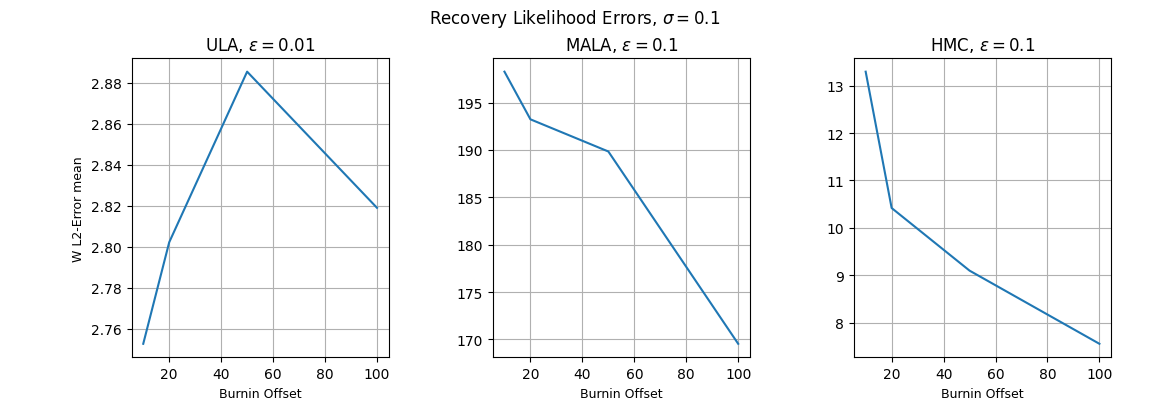
\includegraphics[width=0.85\linewidth]{assets/figures/low_sigma_recov.png}
  	\captionof{figure}{Recovery Likelihood error for $\sigma = 0.1$ against burnin}
  	%\label{fig:Mode_Experiment}
\end{figure}

In that setting, while still performing very poorly, ULA surprisingly performed the best. 
A reason for this could be that the data samples upon which the recovery adapter conditions change at every training iteration.
If $\sigma$ is too small, and the conditional distribution has thus low variance, then changing the samples can potentially shift the mean 
and effectively reset the convergence of the chains. 
Especially for MALA and HMC this could lead to a large number of rejected samples and thus poor sample quality, 
where the chains might remain mostly in their previous modes.

As the parameters diverged for $\sigma = 0.1$ these runs are excluded in the following results.


\subsubsection{Results for ULA}

For larger burnin, recovery likelihood with $\sigma = 0.5$ actually outperformed ML, with both better final errors and a lower standard deviation.
\begin{figure}[H]
  	\centering
  	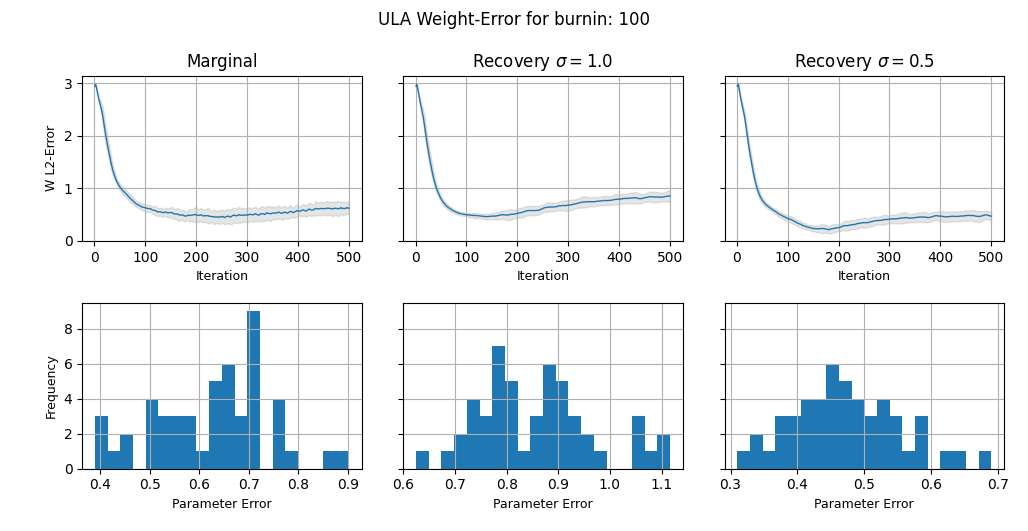
\includegraphics[width=0.85\linewidth]{assets/figures/POLY_ULA_burnin100.png}
  	\captionof{figure}{
		ULA performance across runs. 
		The upper plots represent the entire parameter process, histograms show final error
	}
  	%\label{fig:Mode_Experiment}
\end{figure}

The average error for ML at this setting was at $0.62$ with a standard deviation of $0.11$, 
while RL had an average error of $0.47$ with a standard deviation of $0.08$.
This trend reversed rapidly when decreasing the burnin however, with noticeably worse results for both settings of RL at a burnin lower than $50$.
\begin{figure}[H]
  	\centering
  	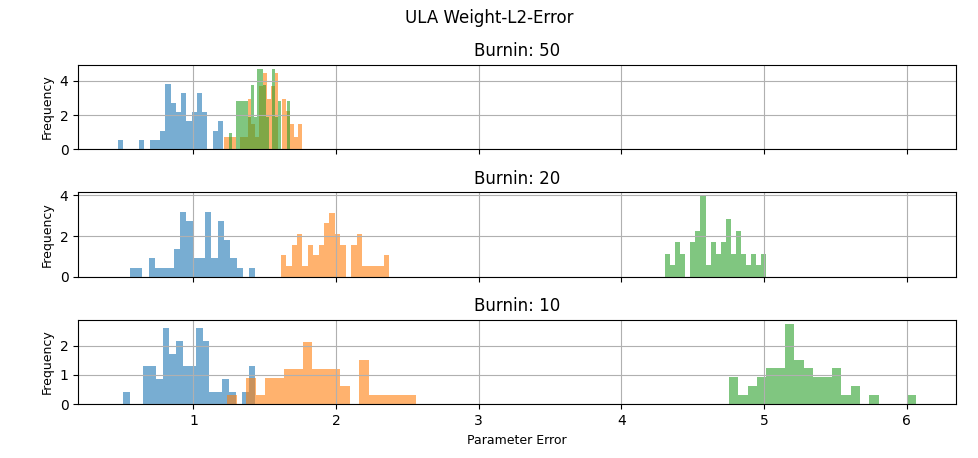
\includegraphics[width=0.85\linewidth]{assets/figures/POLY_ULA_burnins.png}
  	\captionof{figure}{
		ULA performance across runs. 
		Marginal Likelihood (blue), RL with $\sigma = 0.5$ (green), RL with $\sigma = 1.0$ (orange)
	}
  	%\label{fig:Mode_Experiment}
\end{figure}

It is noteworthy that ML didn't suffer as significantly as expected for the lower burnins, although the overall performance was worse using ULA.


\subsubsection{Results for MALA}

The experiments with MALA show a trend for the variance of the RL estimator more clearly.
For a burnin of $100$ the overall estimates are fairly good, but we can see that decreasing $\sigma$ increases the variance of the final estimator.

\begin{figure}[H]
  	\centering
  	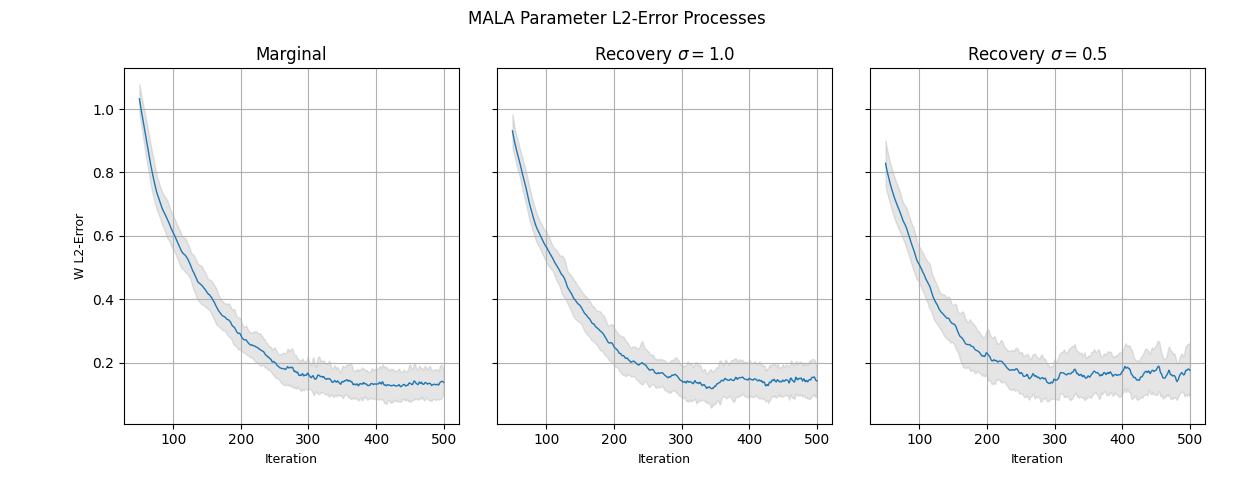
\includegraphics[width=0.85\linewidth]{assets/figures/POLY_MALA_pro100.png}
  	\captionof{figure}{
		MALA processes for burnin $100$.
		RL for $\sigma = 0.5$ shows significantly higher variance
	}
  	%\label{fig:Mode_Experiment}
\end{figure}






\subsection{Multivariate Gaussian Model}

The multivariate Gaussian distribution is unimodal and easy to sample from. 
It serves as a baseline, for which one would expect both ML and RL do perform similarly well in terms of estimate quality.
The test model is two dimensional with target parameters
\[
\begin{aligned}
	\mu &= \begin{pmatrix} 3 \\ 3 \end{pmatrix} \\
	\Sigma &= 
	\begin{pmatrix}
		2 & 0 \\
		0 & 2 \\
	\end{pmatrix} \\
\end{aligned}
\]

and start parameters
\[
\begin{aligned}
	\mu_0 &= \begin{pmatrix} 2 \\ 2 \end{pmatrix} \\
	\Sigma_0 &= 
	\begin{pmatrix}
		2 & 0 \\
		0 & 1 \\
	\end{pmatrix}. \\
\end{aligned}
\]


\subsection{Gaussian Mixture Model}
Target parameters:
\[
\begin{aligned}
	&\mu_1 = \begin{pmatrix} 2 \\ 2 \end{pmatrix}  &\hspace{20pt}  &\mu_2 = \begin{pmatrix} -1 \\ -1 \end{pmatrix} \\
	&\Sigma_1 = 
	\begin{pmatrix}
		2 & 0 \\
		0 & 2 \\
	\end{pmatrix} 
	&\hspace{20pt}
	&\Sigma_2 = 
	\begin{pmatrix}
		1 & 0 \\
		0 & 1 \\
	\end{pmatrix} \\
\end{aligned}
\]
with weights $(w_1, w_2) = ( 0.2, 0.8 )$

Start parameters:
\[
\begin{aligned}
	&\mu_1^0 = \begin{pmatrix} 3 \\ 3 \end{pmatrix}  &\hspace{20pt}  &\mu_2^0 = \begin{pmatrix} 1 \\ 0 \end{pmatrix} \\
	&\Sigma_1^0 = 
	\begin{pmatrix}
		3 & 0 \\
		0 & 1 \\
	\end{pmatrix} 
	&\hspace{20pt}
	&\Sigma_2^0 = 
	\begin{pmatrix}
		2 & 0 \\
		0 & 2 \\
	\end{pmatrix} \\
\end{aligned}
\]
with weights $(w_1, w_2) = ( 0.5, 0.5 )$





\begin{comment}


\begin{table}[H]
\centering
%\csvautotabular{assets/tables/distance_mean_values.csv}
\csvreader[
	tabular = *{6}{|c}|,
	table head = \hline \bfseries {cluster distance} & \bfseries accuracy & \bfseries precision & \bfseries  recall & \bfseries {F1-score} & \bfseries {ROC AUC Score}\\\hline, 
	late after line = \\\hline
	]{assets/tables/distance_mean_values.csv}{}{%
	\csvcoli & \csvcolii & \csvcoliii & \csvcoliv & \csvcolv  & \csvcolvi
}
\caption{Table aggregated by cluster distance}
\end{table}

%----------------------------------------------------------------------------------------------------------------------------------------------------------------------------------------------------
\subsection{Univariate Polynomial}
ULA epsilon = 1e-1 -> NaN cascade
ULA epsilon = 1e-4 -> NaN cascade

%----------------------------------------------------------------------------------------------------------------------------------------------------------------------------------------------------
While there is a lot of theory developed for stochastic processes, 
the complexity contributed by the components of the learning procedure makes it very hard to derive the parameter process analytically.
Even assuming that the samplers for the model provide bona fide samples of the model distribution, 
the randomness of the model samples and of the batch selection comes in in the form of gradients of the likelihood.
It is then warped by the optimisation procedure, which could itself be stochastic algorithm.


Hence there are a lot of dependencies and the evaluation here is empirical and, due to the vast space of hyper parameters and potential choices in strategy,
necessarily not comprehensive.


%----------------------------------------------------------------------------------------------------------------------------------------------------------------------------------------------------
\subsection{Effect of the Sampler-Stepsize} 

The more we decrease $\varepsilon$ the smaller the steps we take in the sampler iterations.
One effect is that it is more likely to get stuck in a vast mode, depending on the distribution.
Another effect is that we decrease the contribution of the gradient compared to the contribution of the random fluctuations.
This is because the square root makes values significantly larger the closer $x$ is to 0.
When considering the stochastic process, which we discretise, this makes intuitive sense.
The more we zoom into the graph of a realisation of an Ito process, the less 'visible' the effect of the drift term becomes, 
and the more pronounced one can observe the erratic behaviour of the Wiener process term.

Suppose we have a distribution with very light tails and that the probability mass is concentrated in a small region, like the one induced by the polynomial energy, 
and that our chain happens to be close to the boundary of the complement of that region in which the energy increases very strongly.
If we choose a large step size the gradient dominates and the steps are big, potentially overcorrecting and moving the chain into a region with very high energy.
But if we choose the step size too low, the stochastic term dominates and can randomly push the chain into a region with very high energy again.
Intuitively this is the reason why the ULA sampler can easily diverge, both for too large and too low step sizes.
\end{comment}
















%\input{content/output}

\begin{comment}
\begin{thebibliography}{9}

\bibitem{SMOTE}
 Nitesh, V., Chawla., Kevin, W., Bowyer., Lawrence, O., Hall., W., Philip, Kegelmeyer. (2002). SMOTE: synthetic minority over-sampling technique. Journal of Artificial Intelligence Research, 16(1):321-357. doi: 10.1613/JAIR.953

\bibitem{ADASYN}
 Haibo He, Yang Bai, E. A. Garcia and Shutao Li, "ADASYN: Adaptive synthetic sampling approach for imbalanced learning," 2008 IEEE International Joint Conference on Neural Networks (IEEE World Congress on Computational Intelligence), Hong Kong, 2008, pp. 1322-1328, doi: 10.1109/IJCNN.2008.4633969.

\end{thebibliography}	
\end{comment}

\section{References}
\bibliographystyle{plain} % We choose the "plain" reference style
\bibliography{assets/references} % Entries are in the refs.bib file






\end{document}
